\documentclass{beamer}
\usepackage[utf8]{inputenc}
\usepackage{amsmath, amssymb, bm}
\usepackage{physics}
\usepackage{graphicx}
\usepackage{hyperref}
\usepackage{xmpmulti}
\usepackage{tikz}
\usepackage{pgfplots}
\pgfplotsset{compat=newest}
\usepackage{siunitx}
\usepackage{longtable}
\sisetup{round-mode=places,round-precision=1}


\usetheme{Madrid} % You can change the theme as you like
\usecolortheme{seagull}





\begin{document}

\title[Quantum Computing and ML]{\textbf{Quantum Technologies, risks and prospects}}
\author{Morten Hjorth-Jensen}
\institute{Department of Physics and Center for Computing in Science Education, University of Oslo, Norway}
\date{40th Nordic Conference on Law and IT – Regulating for Complexity, November 5-7, 2025}


%-----------------------------------------------------------
%\begin{frame}
%    \titlepage
%\end{frame}

%-----------------------------------------------------------


\begin{frame}[plain,fragile]
\titlepage
\end{frame}

\section{Introduction to quantum technologies}
\begin{frame}[plain,fragile]
\frametitle{What is this talk about?}

\begin{block}{}
In this seminar I will try to give a pedestrian yet comprehensive overview of the fundamental principles underpinning quantum technologies. Beginning with the essential quantum concepts that form their theoretical foundation, I will examine how these ideas are translated into contemporary technological applications. The discussion will further address the interplay between scientific advances and current public and private investments in the field, providing an outlook on prospective developments over the coming decade. Finally, I will consider a range of ethical and legal challenges that accompany the ongoing expansion of quantum technologies.
And why this could (or should) be of interest to a society as a whole. 
\end{block}

\end{frame}

\begin{frame}[plain,fragile]
\frametitle{Quantum technologies and machine learning/AI are tighly interwoven }


% inline figure
\centerline{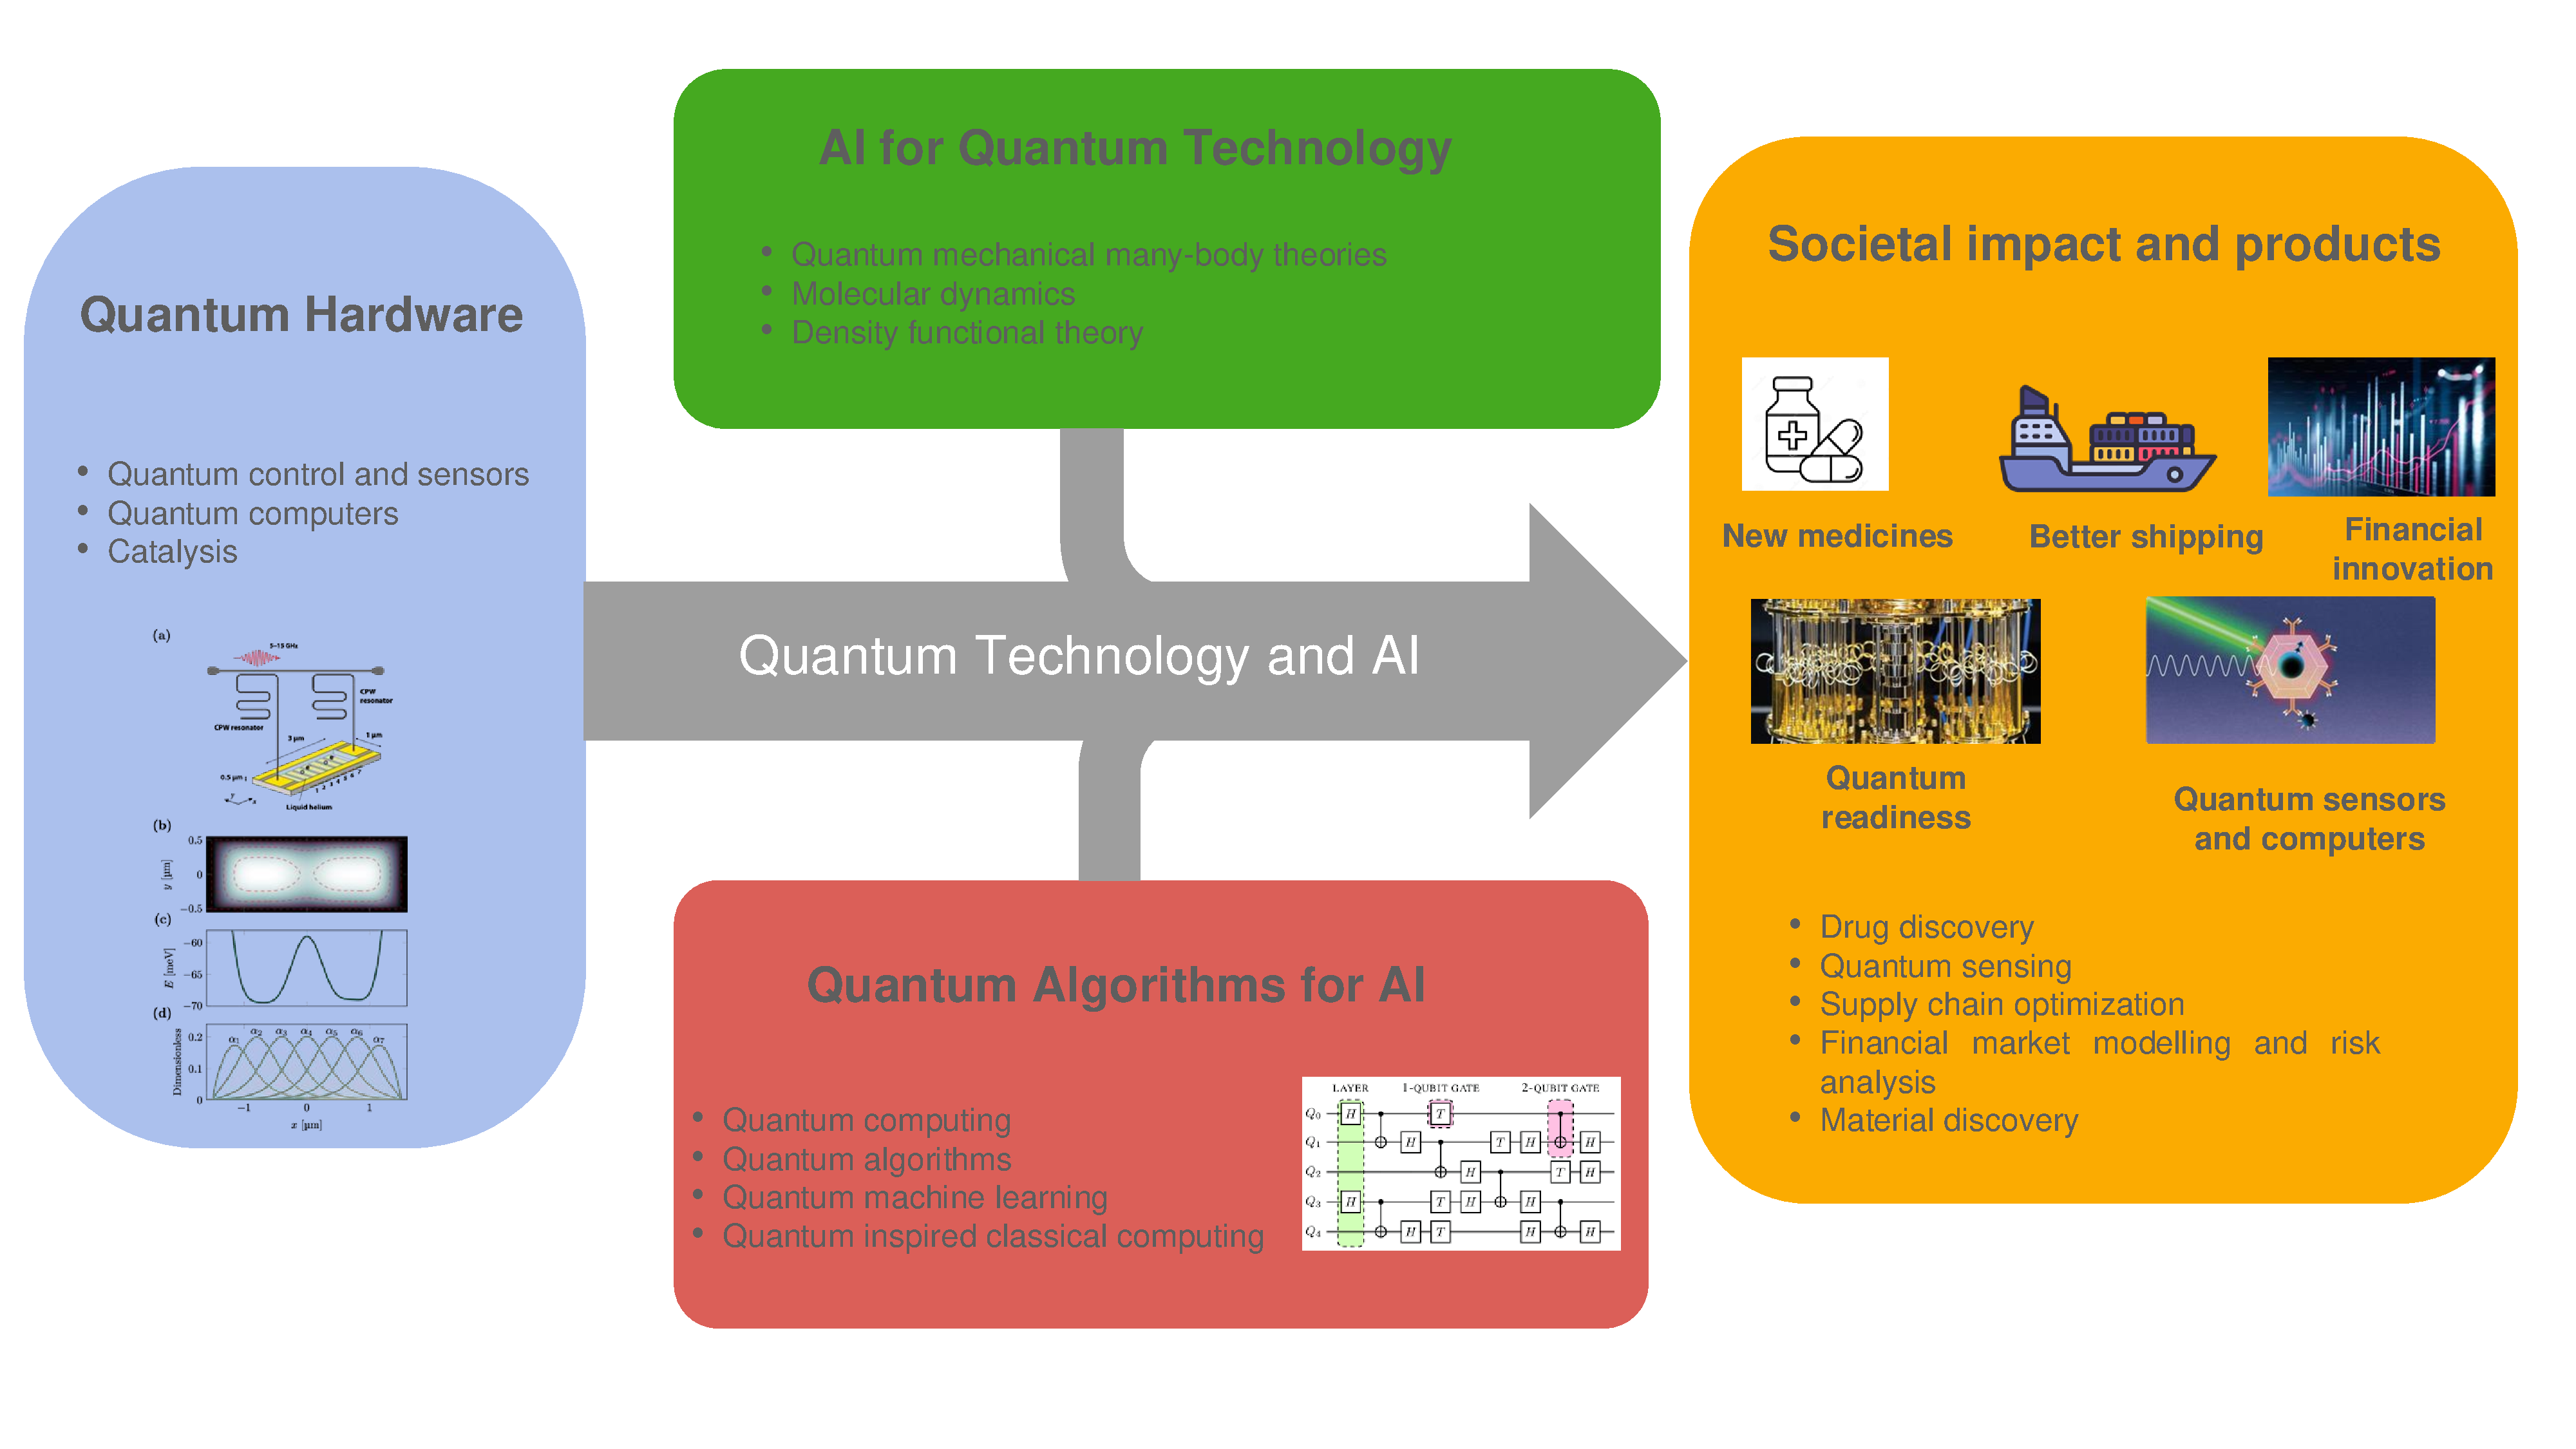
\includegraphics[width=1.05\linewidth]{figures/figureintro.pdf}}

\end{frame}


\begin{frame}[plain,fragile]
\frametitle{From Moore's law to Huang's law, the race for more performance}

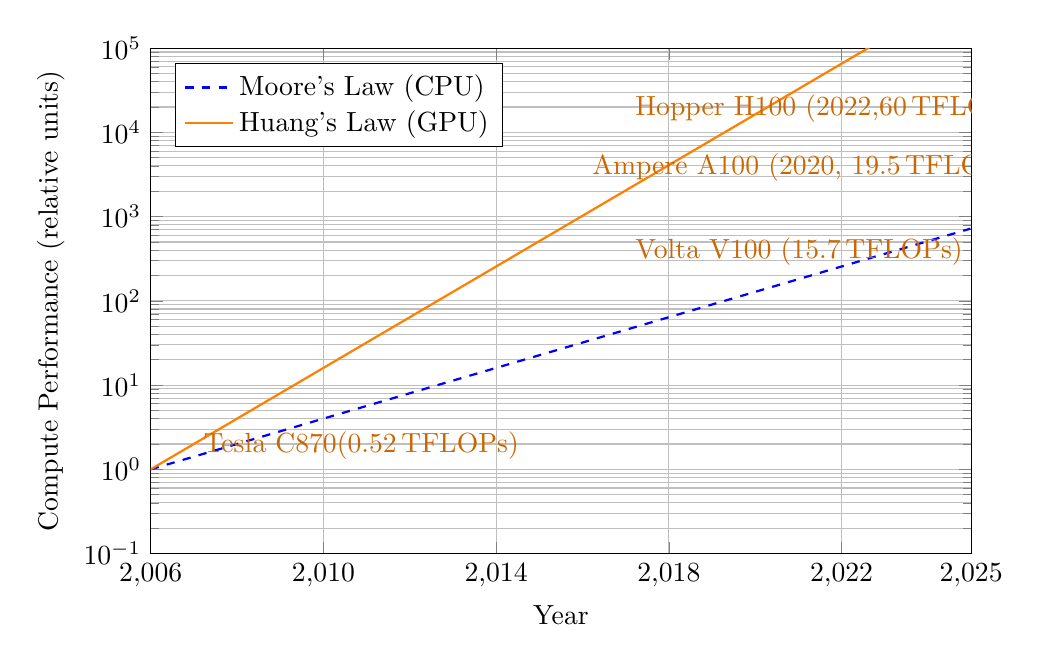
\begin{tikzpicture}
  \begin{semilogyaxis}[
    width=12cm, height=8cm,
    xlabel={Year},
    ylabel={Compute Performance (relative units)},
    xmin=2006, xmax=2025,
    ymin=0.1, ymax=1e5,
    xtick={2006,2010,2014,2018,2022,2025},
    grid=both,
    legend pos=north west,
    legend cell align=left,
    every axis plot/.append style={thick}
  ]

  % Moore's Law (doubling every two years)
  \addplot[
    blue, dashed, domain=2006:2025, samples=200
  ] {2^((x-2006)/2)};
  \addlegendentry{Moore's Law (CPU)}

  % Huang's Law (doubling every year)
  \addplot[
    orange, domain=2006:2025, samples=200
  ] {2^(x-2006)};
  \addlegendentry{Huang's Law (GPU)}

  % GPU Milestones
  \node[anchor=south west,orange!80!black] at (axis cs:2007,1) {Tesla C870(\SI{0.52}{TFLOPs})};
  \node[anchor=south west,orange!80!black] at (axis cs:2017,200) {Volta V100 (\SI{15.7}{TFLOPs})};
  \node[anchor=south west,orange!80!black] at (axis cs:2016,2000) {Ampere A100 (2020, \SI{19.5}{TFLOPs})};
  \node[anchor=south west,orange!80!black] at (axis cs:2017,10000) {Hopper H100 (2022,\SI{60}{TFLOPs})};
  \end{semilogyaxis}
\end{tikzpicture}

\end{frame}
e


\begin{frame}[plain,fragile]
\frametitle{Machine learning and AI models are computationally expensive}


% inline figure
\centerline{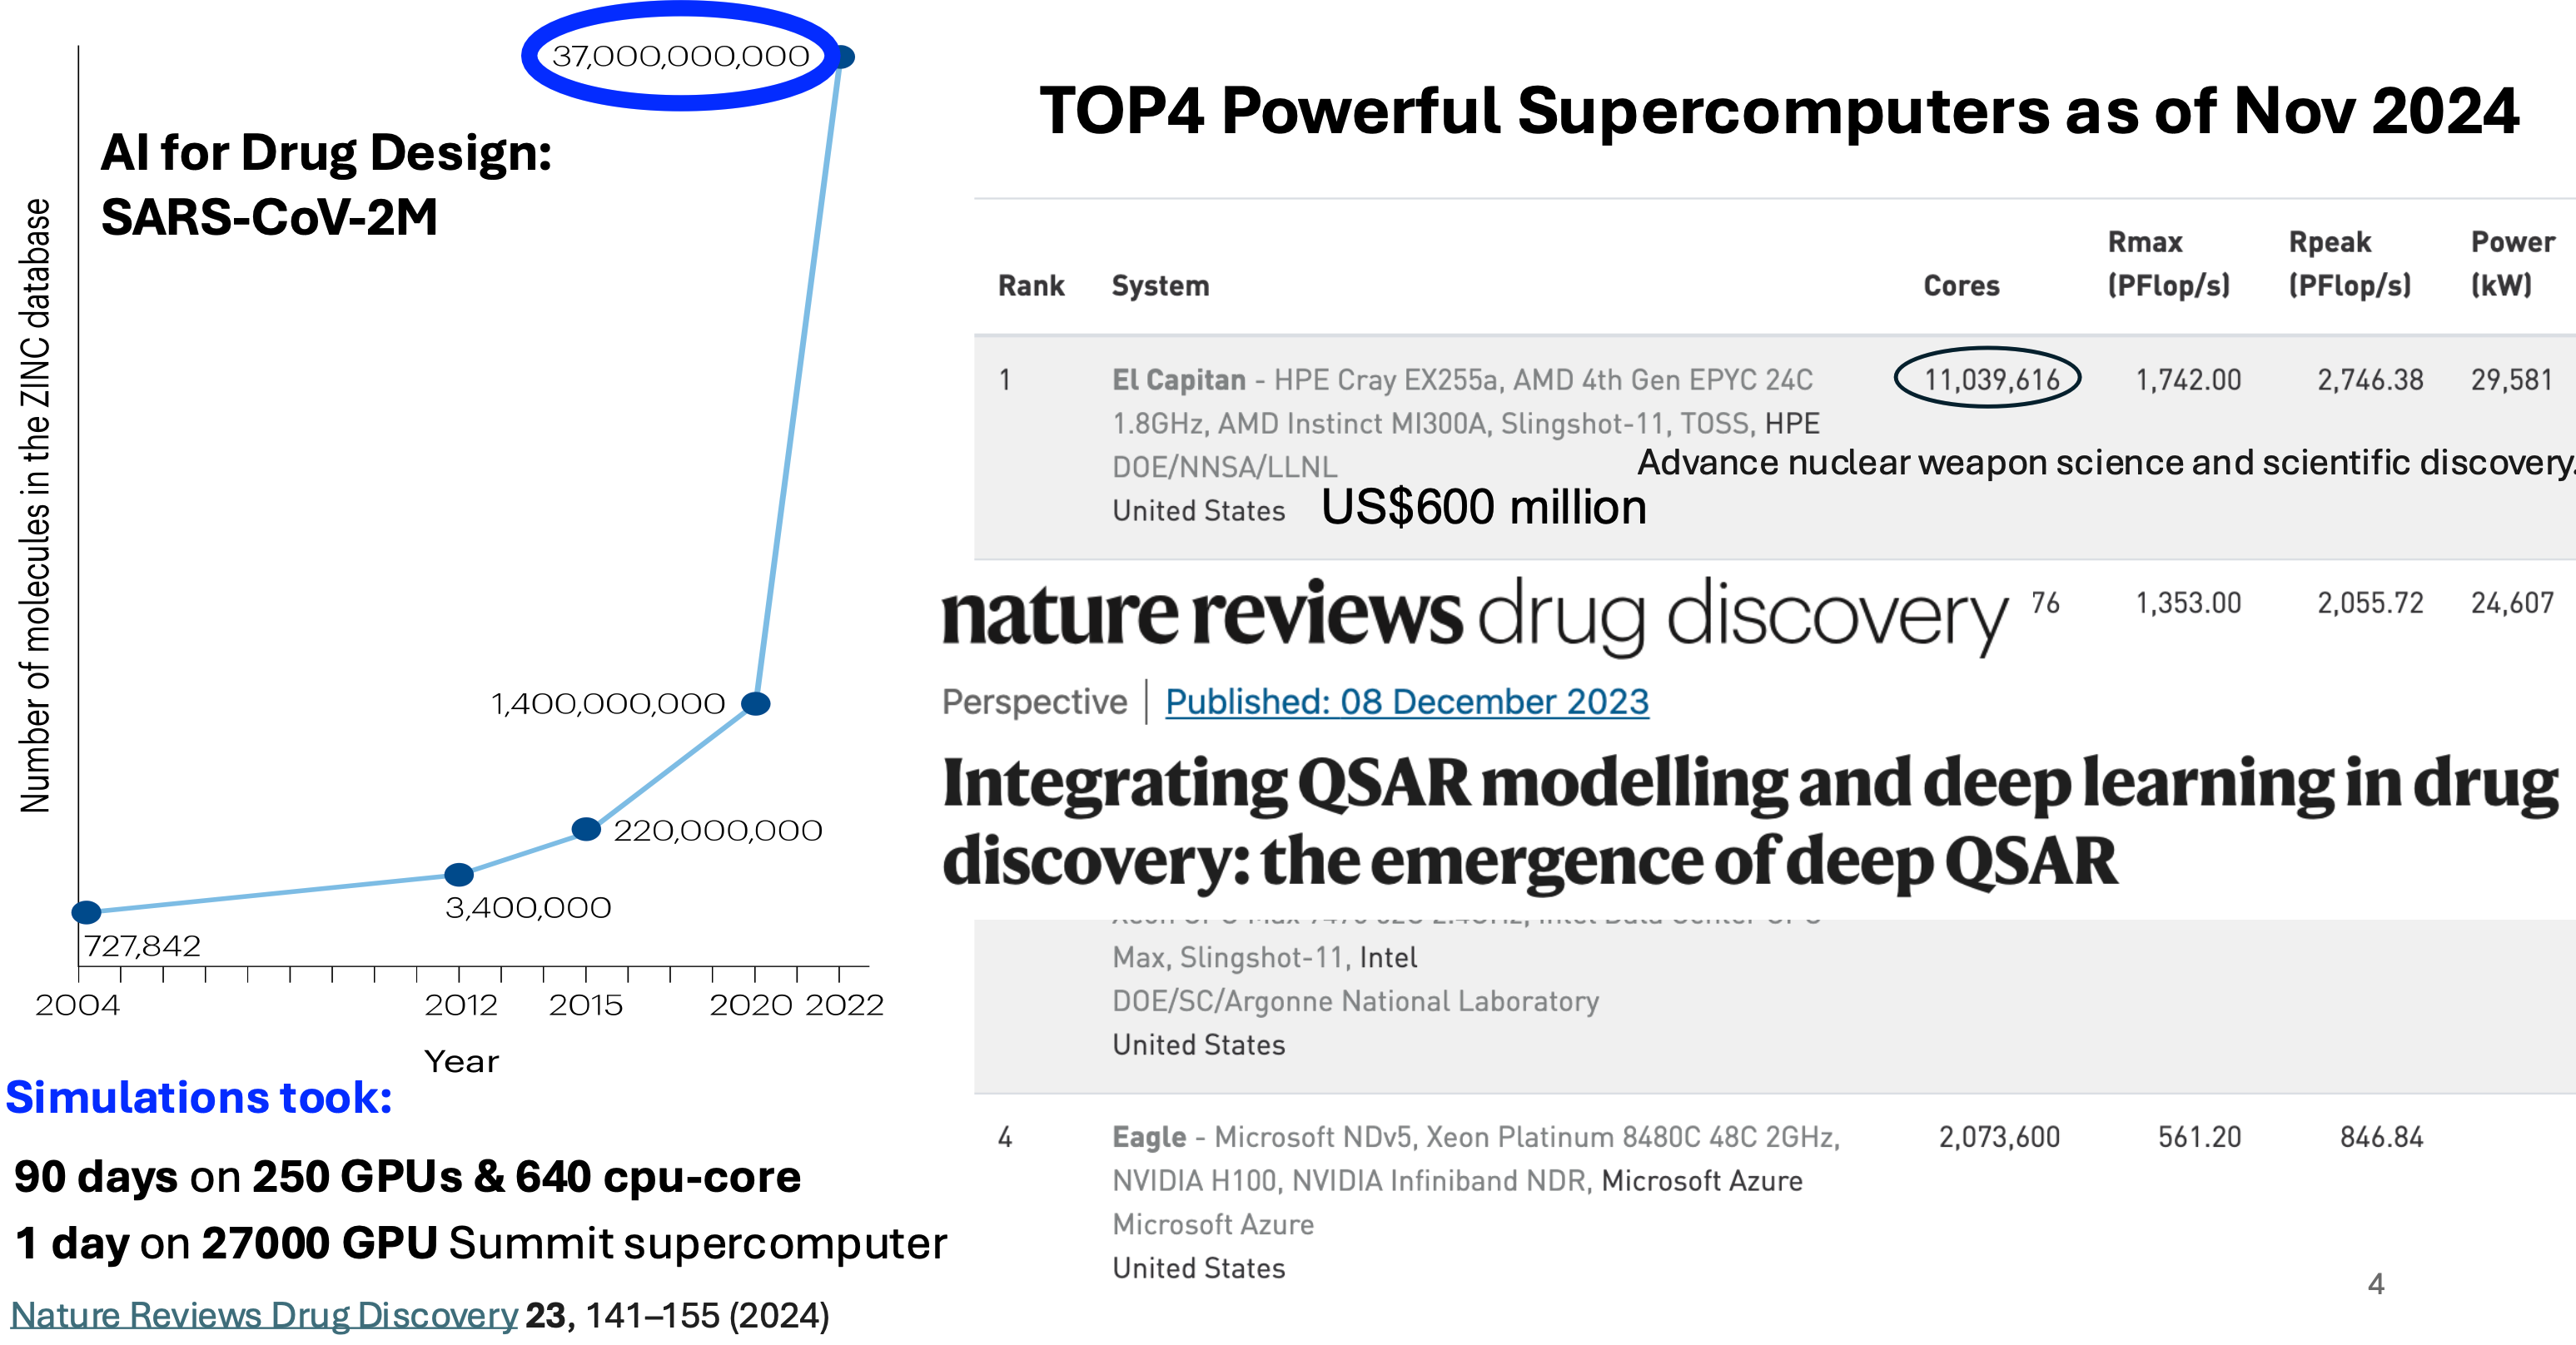
\includegraphics[width=1.0\linewidth]{figures/aitalk2.png}}

\end{frame}


\begin{frame}[plain,fragile]
\frametitle{And power greedy, perhaps quantum computers can reduce the impact?}

% inline figure
\centerline{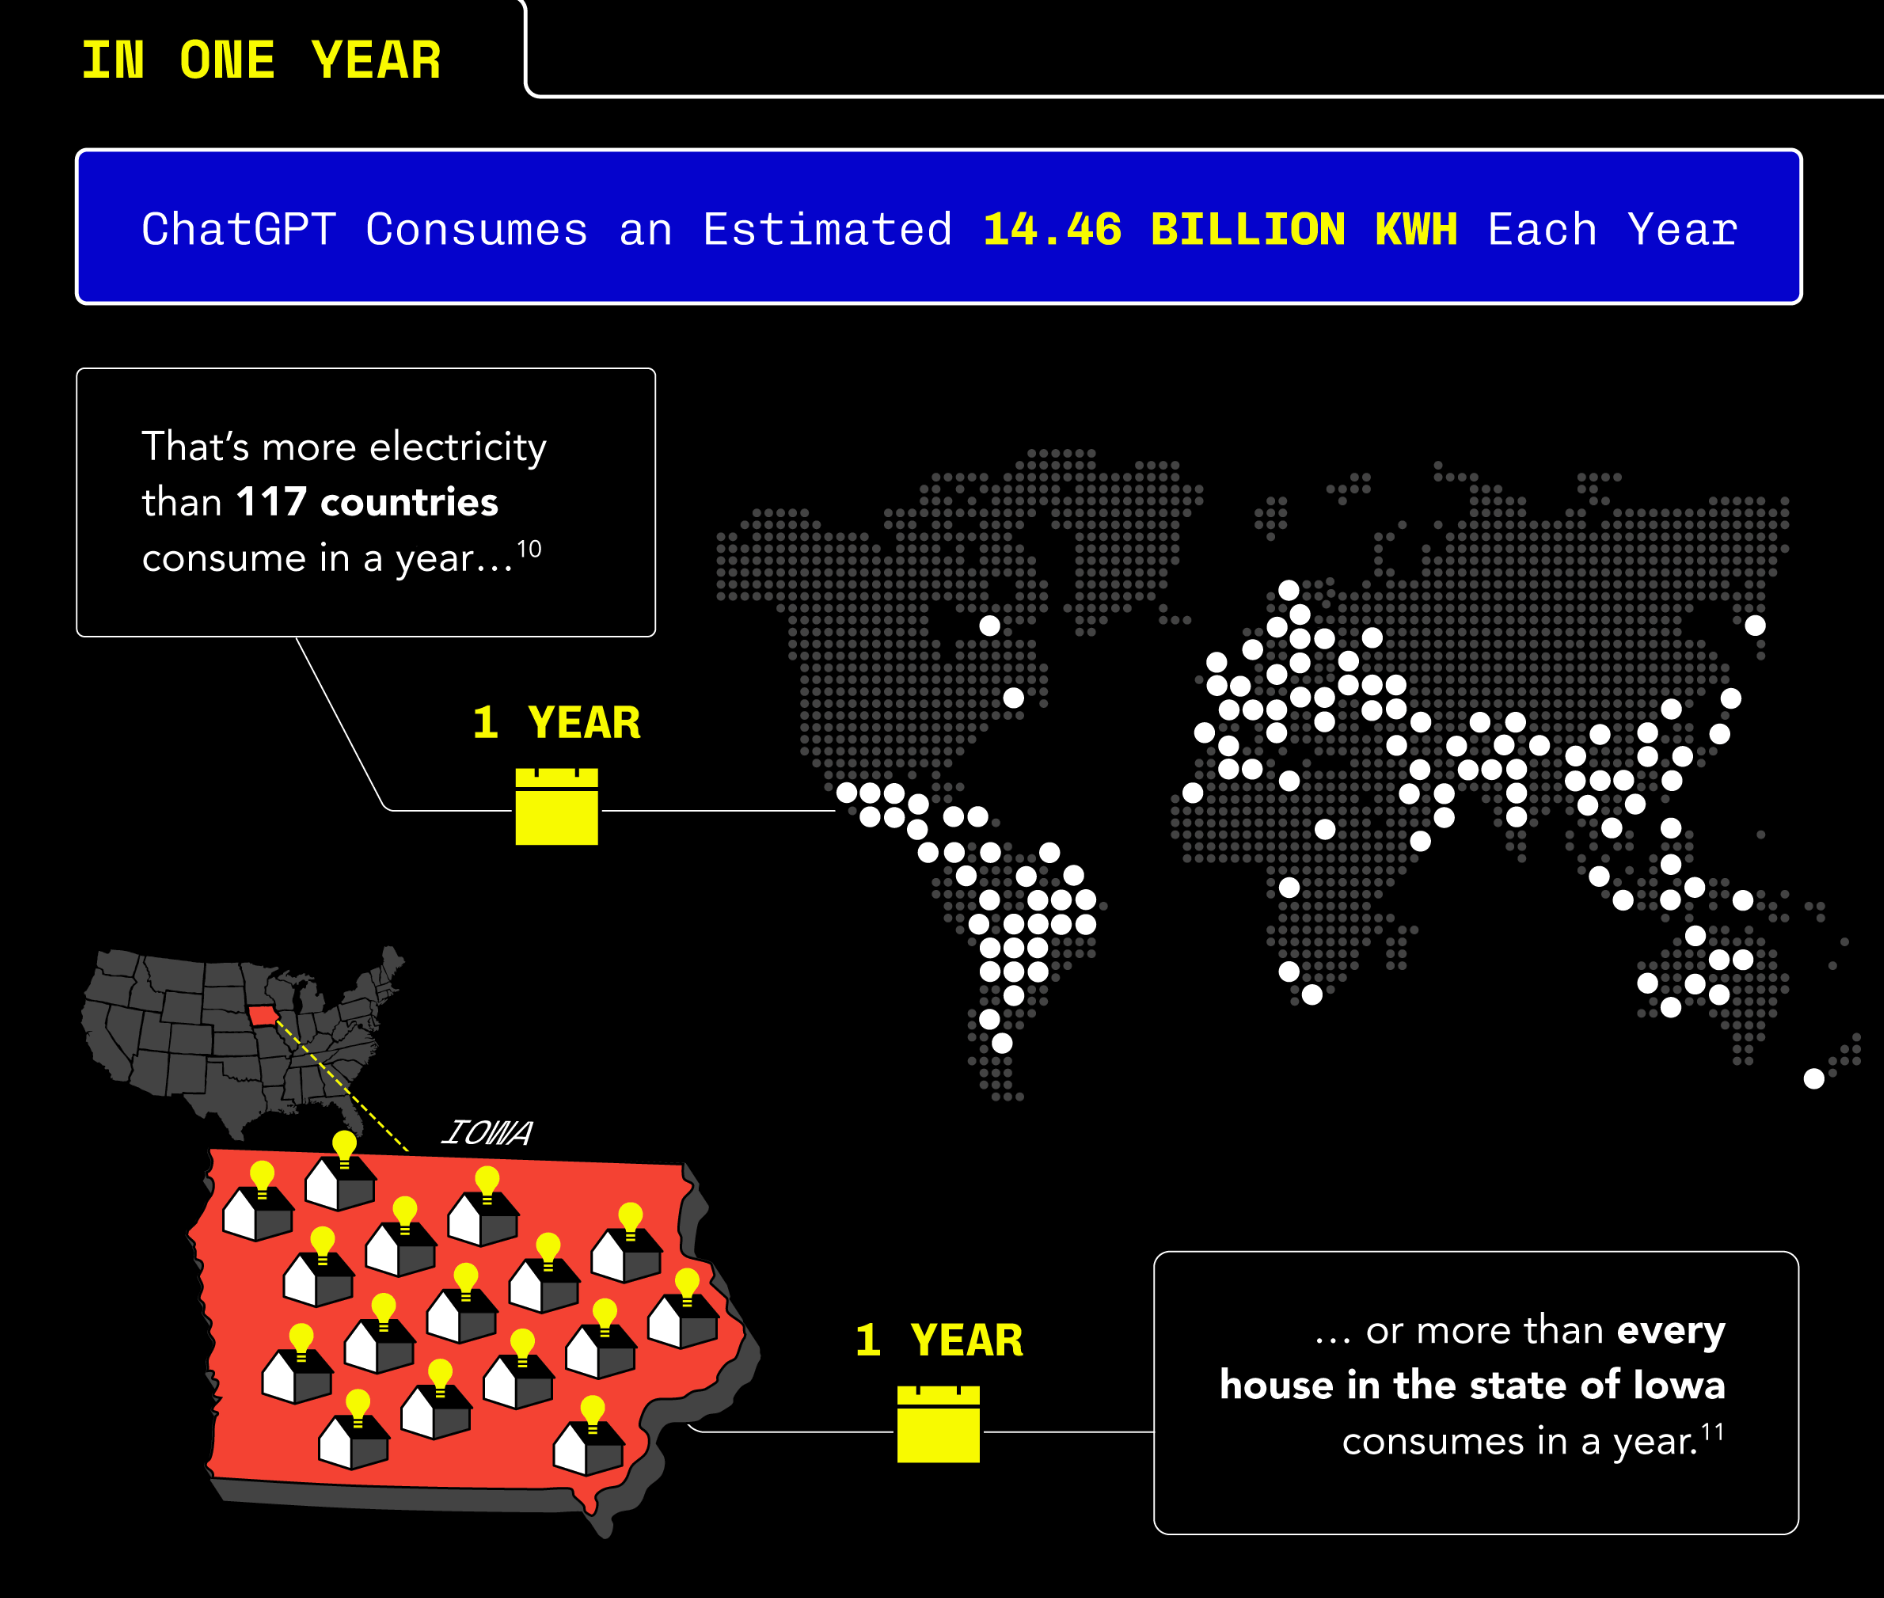
\includegraphics[width=0.7\linewidth]{figures/aitalk1.png}}
Taken from \url{https://www.businessenergyuk.com/knowledge-hub/chatgpt-energy-consumption-visualized/}
\end{frame}

\begin{frame}
\framtitle{And not exactly environmetally friendly}
\begin{itemize}
\item In Ireland, data centers consume more than 20 percent of the country’s electricity.
\item In Chile, precious aquifers are in danger of depletion.
\item In South Africa, where blackouts have long been routine, data centers are further taxing the national grid.
\item Similar concerns have surfaced in Brazil, Britain, India, Malaysia, the Netherlands, Singapore and Spain
\end{itemize}
\end{frame}

\begin{frame}[plain,fragile]
\frametitle{The future is here, sooner than we may think}


% inline figure
\centerline{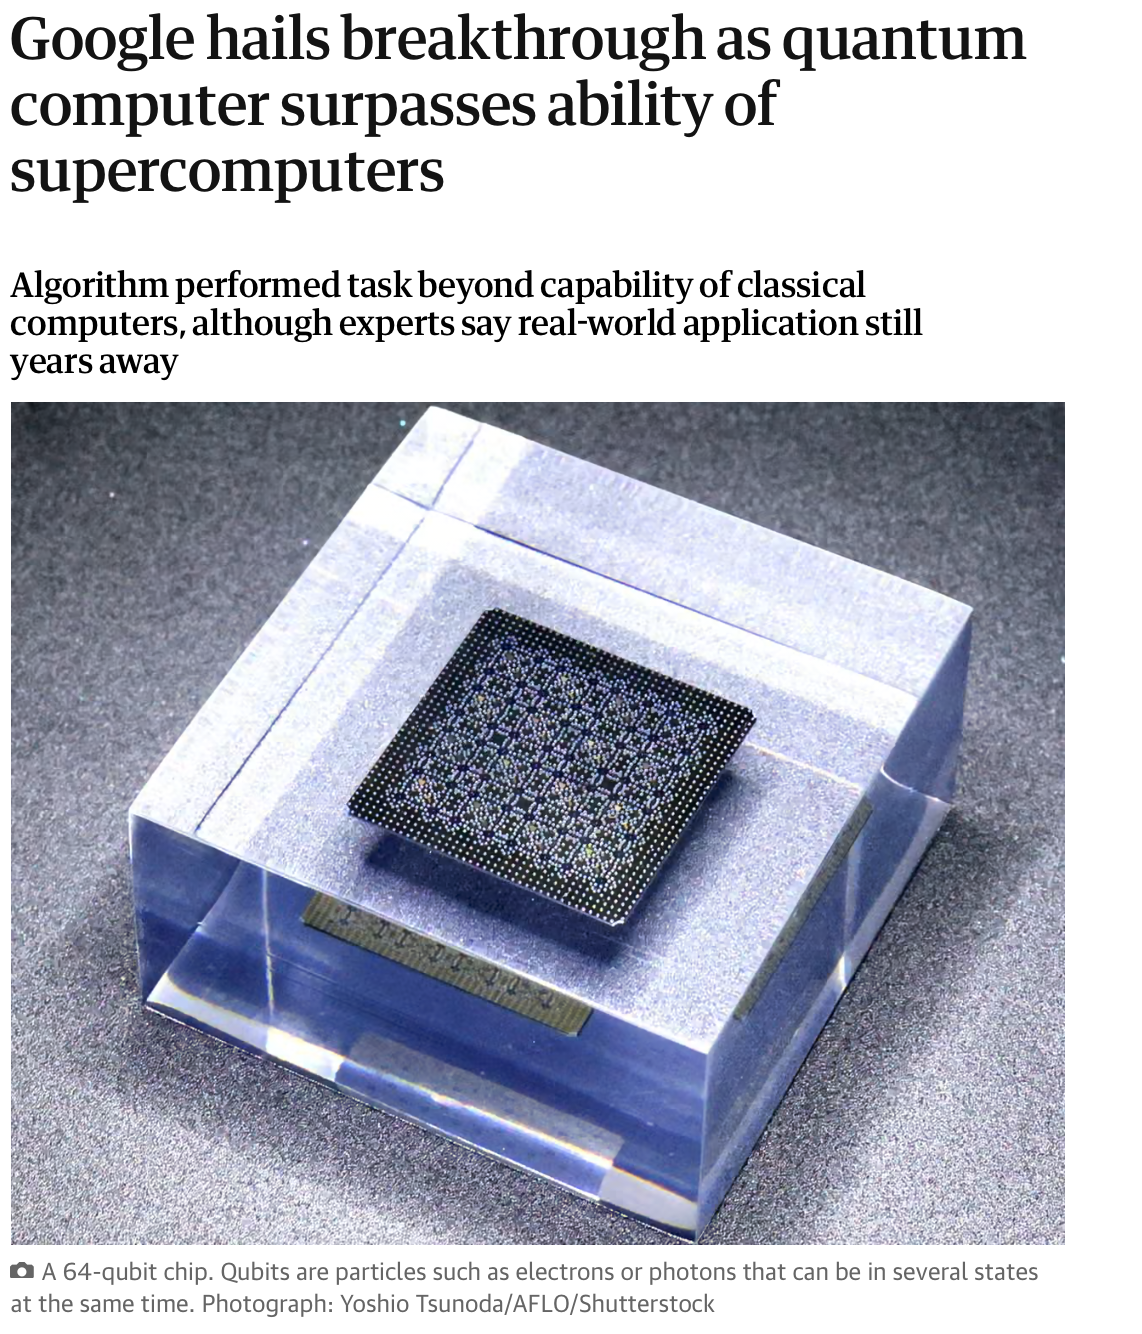
\includegraphics[width=1.05\linewidth]{figures/figuregoogle.png}}

\end{frame}

\begin{frame}[plain,fragile]
\frametitle{Add info about tech regulations in AI}
US-China war on restriciting access to sophisticated technologies
\begin{enumerate}
\item TSMC restrictions
\item Seagate, Micron
\item Huawei, Nvidia etc, semiconductor control etc
\end{enumerate}
Mention Alessandro Aresu's book
\end{frame}




%-----------------------------------------------------------
%\section{Introduction to Quantum Computing}
\begin{frame}{The basis: What is Quantum Computing?}
Quantum computing leverages principles of quantum mechanics to perform computations beyond classical capabilities.

\vspace{10pt}
\textbf{Key Concepts:}
\begin{itemize}
\item \textbf{Superposition:} Qubits can exist in a combination of states.
\item \textbf{Entanglement:} Correlation between qubits regardless of distance.
\item \textbf{Quantum Interference:} Probability amplitudes interfere to solve problems.
\end{itemize}

%\textbf{Qubit Representation:}
%\[
%\ket{\psi} = \alpha \ket{0} + \beta \ket{1}, \quad |\alpha|^2 + |\beta|^2 = 1
%\]
\end{frame}



%\section{Quantum Speedups}
\begin{frame}{Quantum Speedups}
\textbf{Why Quantum?}
\begin{itemize}
    \item \textbf{Quantum Parallelism:} Process multiple states simultaneously.
    \item \textbf{Quantum Entanglement:} Correlated states for richer information.
    \item \textbf{Quantum Interference:} Constructive and destructive interference to enhance solutions.
\end{itemize}

\textbf{Example - Grover's Algorithm:}
\[
\text{Quantum Search Complexity: } O(\sqrt{N}) \text{ vs. } O(N)
\]

\textbf{Advantage:}
- Speedups in high-dimensional optimization and linear algebra problems.
\end{frame}

%-----------------------------------------------------------
%\section{Challenges in Quantum Machine Learning}
\begin{frame}{Challenges and Limitations}
\textbf{1. Quantum Hardware Limitations:}
\begin{itemize}
    \item Noisy Intermediate-Scale Quantum (NISQ) devices.
    \item Decoherence and limited qubit coherence times.
\end{itemize}

\textbf{2. Data Encoding:}
\begin{itemize}
    \item Efficient embedding of classical data into quantum states.
\end{itemize}

\textbf{3. Scalability:}
\begin{itemize}
    \item Difficult to scale circuits to large datasets.
\end{itemize}
\end{frame}




\begin{frame}{What is Quantum Entanglement?}
\textbf{Quantum Entanglement} is a quantum phenomenon where two or more particles become correlated in such a way that the state of one particle directly affects the state of the other, regardless of distance.

\vspace{10pt}
\textbf{Key Features:}
\begin{itemize}
    \item Non-local correlations
    \item No classical analog
    \item Violates Bell's inequalities
\end{itemize}

\textbf{Entangled State Example:}
\[
\ket{\Phi^+} = \frac{1}{\sqrt{2}} (\ket{00} + \ket{11})
\]

\end{frame}


\begin{frame}{1. Quantum Communication}
\textbf{Quantum Teleportation:}
\begin{itemize}
    \item Entanglement enables the transmission of quantum states using classical communication.
    \item No need to send the physical quantum particle.
\end{itemize}

\textbf{Advantage:}
\begin{itemize}
\item Instantaneous state transfer within quantum mechanics constraints.
\item Quantum networks rely on entanglement for secure communication.
  \end{itemize}
\end{frame}

\begin{frame}{2. Quantum Cryptography}
\textbf{Quantum Key Distribution:}
\begin{itemize}
    \item Entanglement ensures secure communication.
    \item Eavesdropping disturbs quantum states, revealing interception attempts.
\end{itemize}

\begin{itemize}
\item Any measurement by a third party collapses the wavefunction.  
\item Ensures security based on quantum mechanics, not computational hardness.
\end{itemize}
\textbf{Advantage:} Unconditional security guaranteed by the laws of physics.
\end{frame}

\begin{frame}{3. Quantum Computing}
\textbf{Speedup in Quantum Algorithms:}
\begin{itemize}
    \item Entanglement provides exponential state space.
    \item Quantum parallelism arises from entangled qubits.
\end{itemize}

\textbf{Grover's Algorithm:}
\[
\mathcal{O}(\sqrt{N}) \text{ vs. } \mathcal{O}(N)
\]

\textbf{Shor's Algorithm:}
\[
\text{Factoring in } \mathcal{O}((\log N)^3)
\]
\end{frame}

\begin{frame}[plain,fragile]
\frametitle{4. Quantum Metrology}

\textbf{Quantum Metrology:}
\begin{itemize}
    \item Uses entangled states for ultra-precise measurements.
    \item Overcomes the classical shot-noise limit.
\end{itemize}

\textbf{Heisenberg Limit:}
\[
\Delta \theta \ge \frac{1}{N},
\]

where \( N \) is the number of entangled particles.  

\begin{block}{Advantage:}
\begin{itemize}
\item Quantum entanglement improves sensitivity beyond classical limits.
\end{itemize}
\end{block}
\end{frame}

\begin{frame}{Challenges of Quantum Entanglement}
\textbf{Decoherence:}
\begin{itemize}
    \item Entangled states are fragile.
    \item Interaction with the environment collapses the wavefunction.
\end{itemize}

\textbf{Scalability:}
\begin{itemize}
    \item Difficult to entangle large numbers of qubits.
    \item Error correction requires complex protocols.
\end{itemize}

\textbf{Measurement Problem:}
\begin{itemize}
    \item Measurement destroys entanglement.
    \item Trade-off between information gain and entanglement preservation.
\end{itemize}
\end{frame}

%-----------------------------------------------------------
%\section{Quantum Machine Learning (QML)}
\begin{frame}{What is Quantum Machine Learning?}
\textbf{Quantum Machine Learning (QML)} integrates quantum computing with machine learning algorithms to exploit quantum advantages.

\vspace{10pt}
\textbf{Motivation:}
\begin{itemize}
    \item High-dimensional Hilbert spaces for better feature representation.
    \item Quantum parallelism for faster computation.
    \item Quantum entanglement for richer data encoding.
\end{itemize}


\end{frame}



\begin{frame}[plain,fragile]
\frametitle{Di Vincenzo criteria}

\begin{alertblock}{Quantum computing requirements }
\begin{enumerate}
\item A scalable physical system with well-characterized qubit

\item The ability to initialize the state of the qubits to a simple fiducial state

\item Long relevant Quantum coherence times longer than the gate operation time

\item A \textbf{universal} set of quantum gates

\item A qubit-specific measurement capability
\end{enumerate}

\noindent
\end{alertblock}
\end{frame}


\section{The next decade}

\begin{frame}[plain,fragile]
\frametitle{Considerable investements (add source)}


% inline figure
\centerline{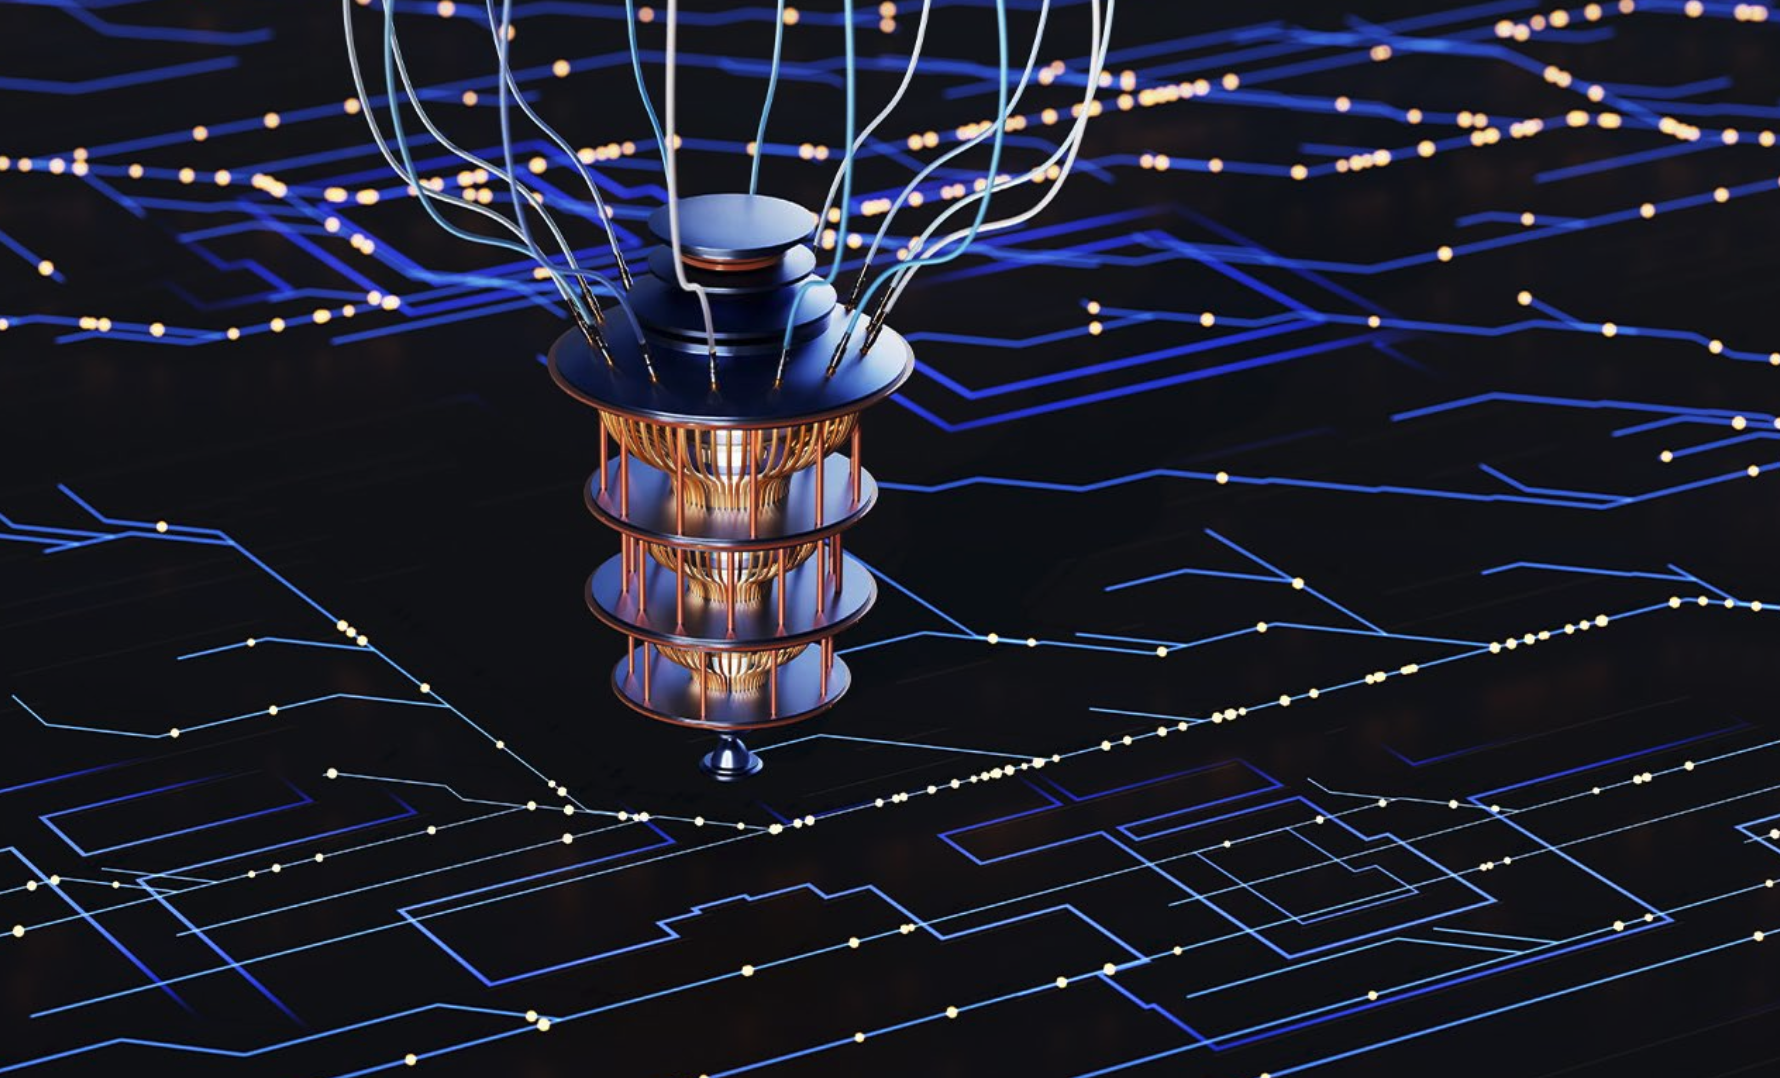
\includegraphics[width=0.9\linewidth]{qcfigures/image1.png}}

\end{frame}


\begin{frame}[plain,fragile]
\frametitle{Considerable investements (add source)}


% inline figure
\centerline{
\includegraphics[width=0.9\linewidth]{qcfigures/image2.png}}

\end{frame}

\begin{frame}[plain,fragile]
\frametitle{Considerable investements (add source)}


% inline figure
\centerline{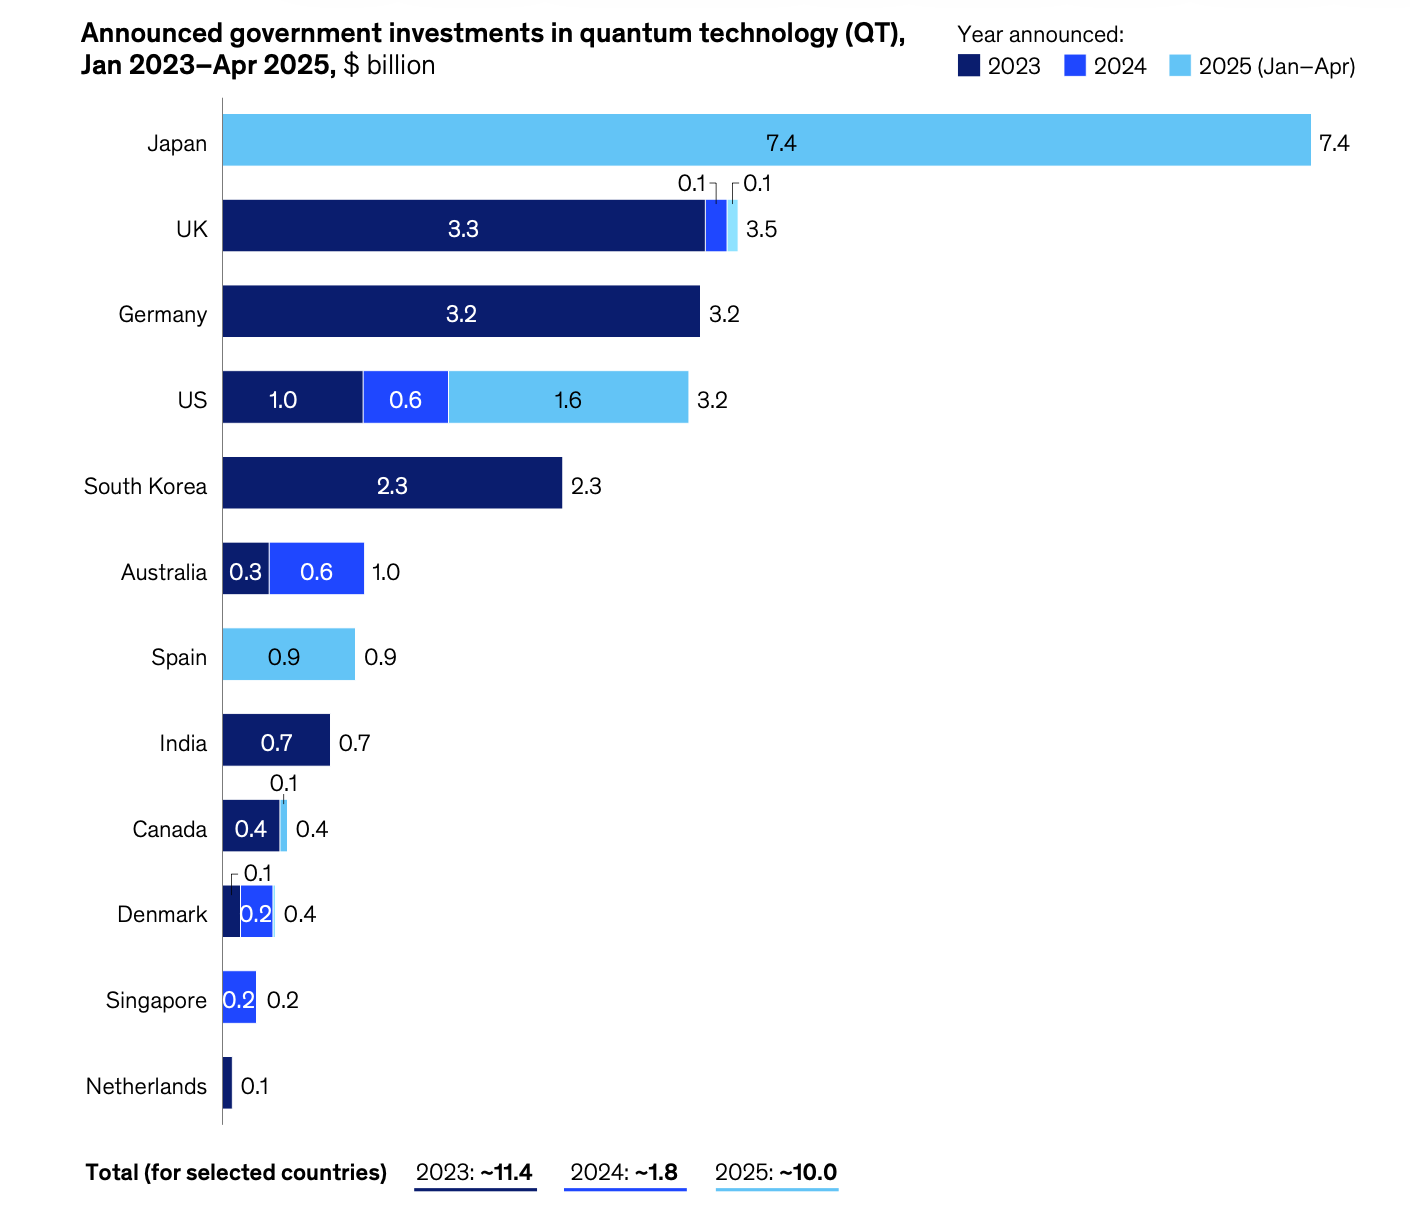
\includegraphics[width=0.9\linewidth]{qcfigures/image3.png}}

\end{frame}

\begin{frame}[plain,fragile]
\frametitle{Considerable investements (add source)}


% inline figure
\centerline{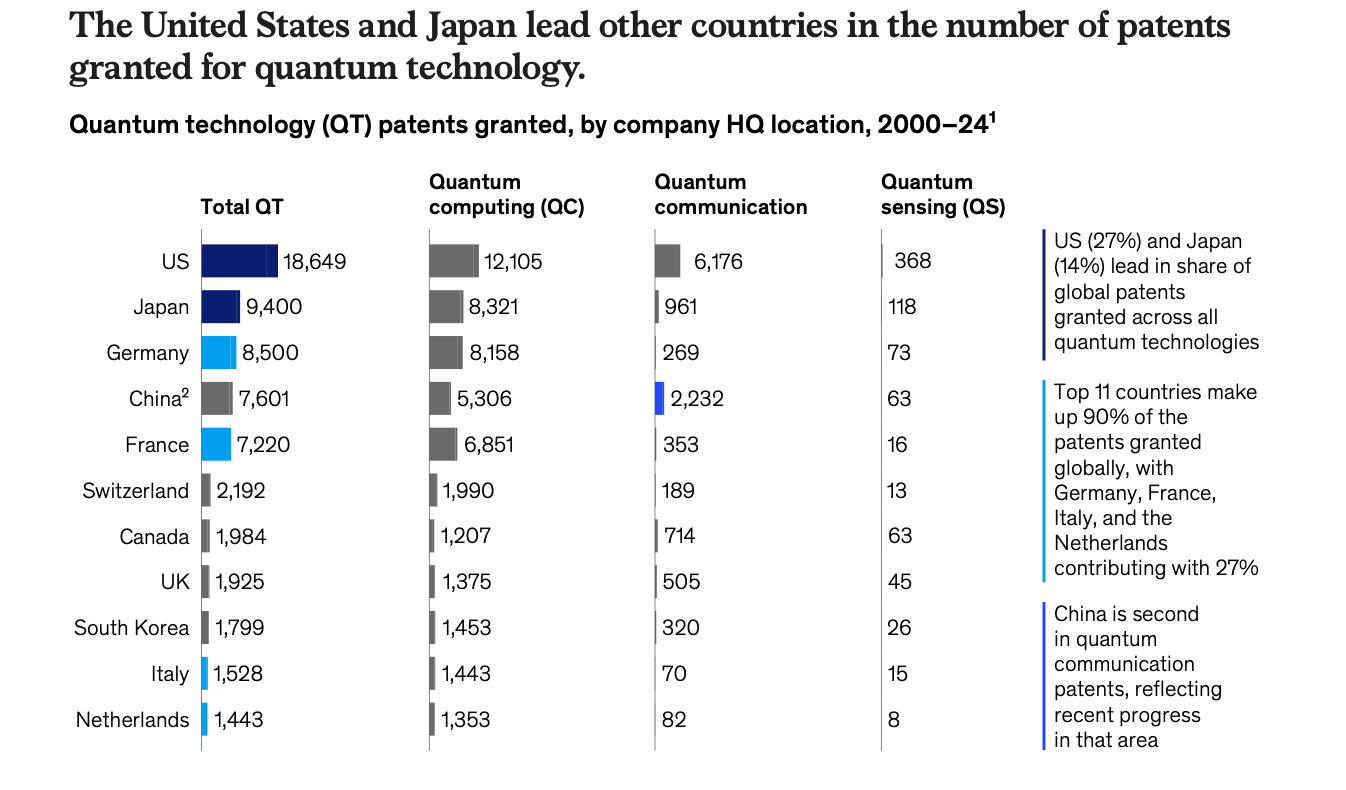
\includegraphics[width=1.0\linewidth]{qcfigures/image4.png}}

\end{frame}

\begin{frame}[plain,fragile]
\frametitle{Considerable investements (add source)}


% inline figure
\centerline{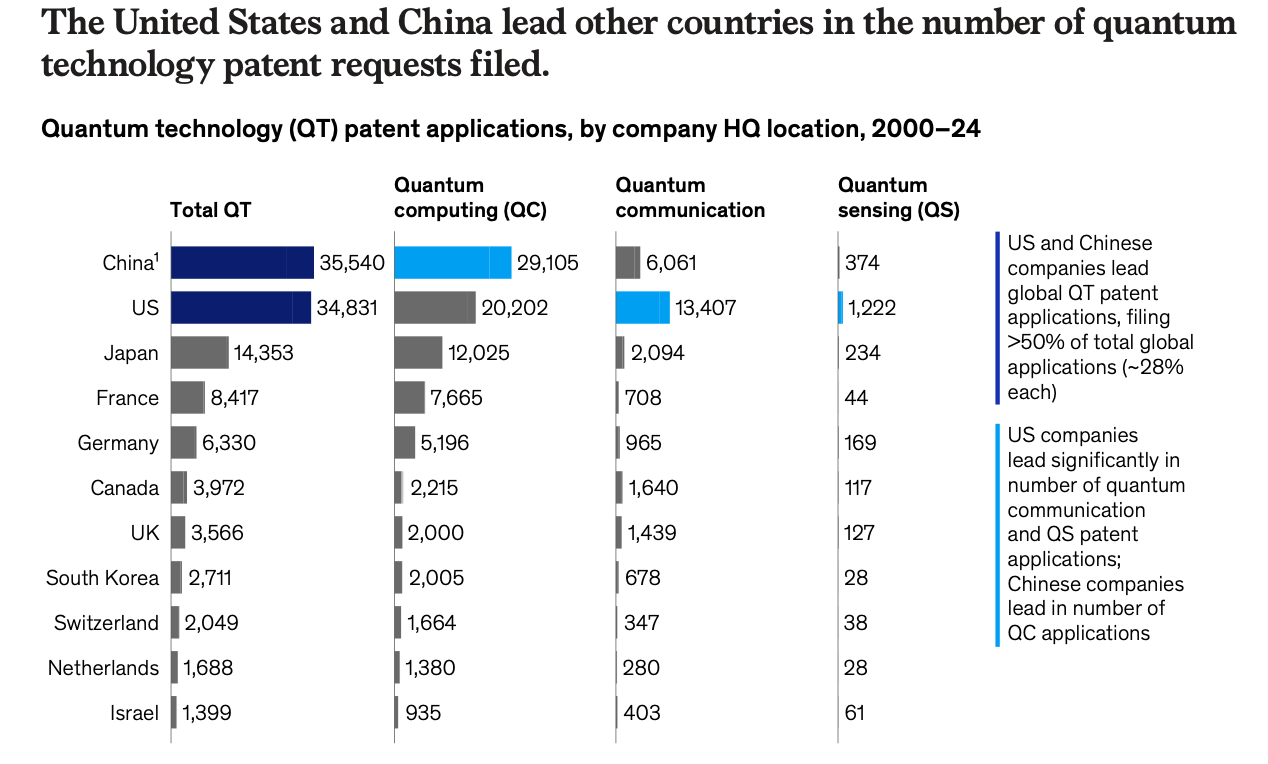
\includegraphics[width=1.0\linewidth]{qcfigures/image5.png}}

\end{frame}


\begin{frame}[plain,fragile]
\frametitle{Considerable investements (add source)}


% inline figure
\centerline{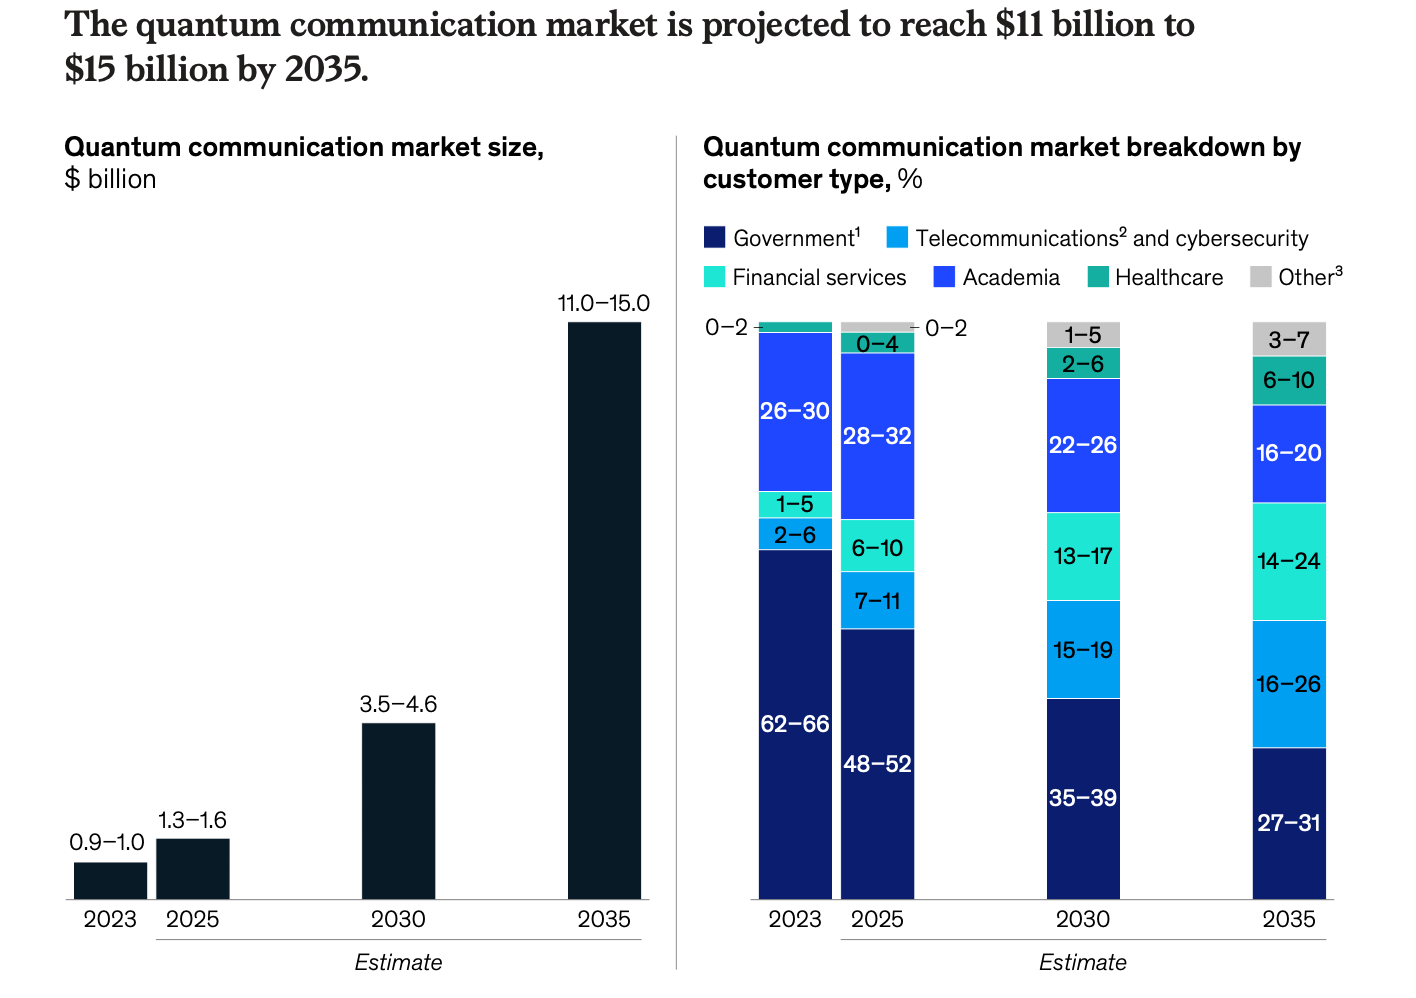
\includegraphics[width=0.9\linewidth]{qcfigures/image6.png}}

\end{frame}



    

\section{Legal aspects and export control resrictions}

\begin{frame}[plain,fragile]
\frametitle{Quantum platforms}

\begin{enumerate}
\item Superconduting qubits
\item Ion traps
\item Quantum dot systems (in semiconductors)
\item more text to come

\end{enumerate}


\end{frame}


\frame
    {
      \frametitle{Important properties, electrons on helium}

      \begin{footnotesize}
     \begin{columns}
       \column{5.0cm}
\begin{enumerate}
\item Long coherence times

\item Highly connect qubits

\item Many qubits in a small area

\item CMOS compatible

\item Fast gates
\end{enumerate}

\column{6cm}
      \begin{center}
        \rotatebox[origin=c]{-90}{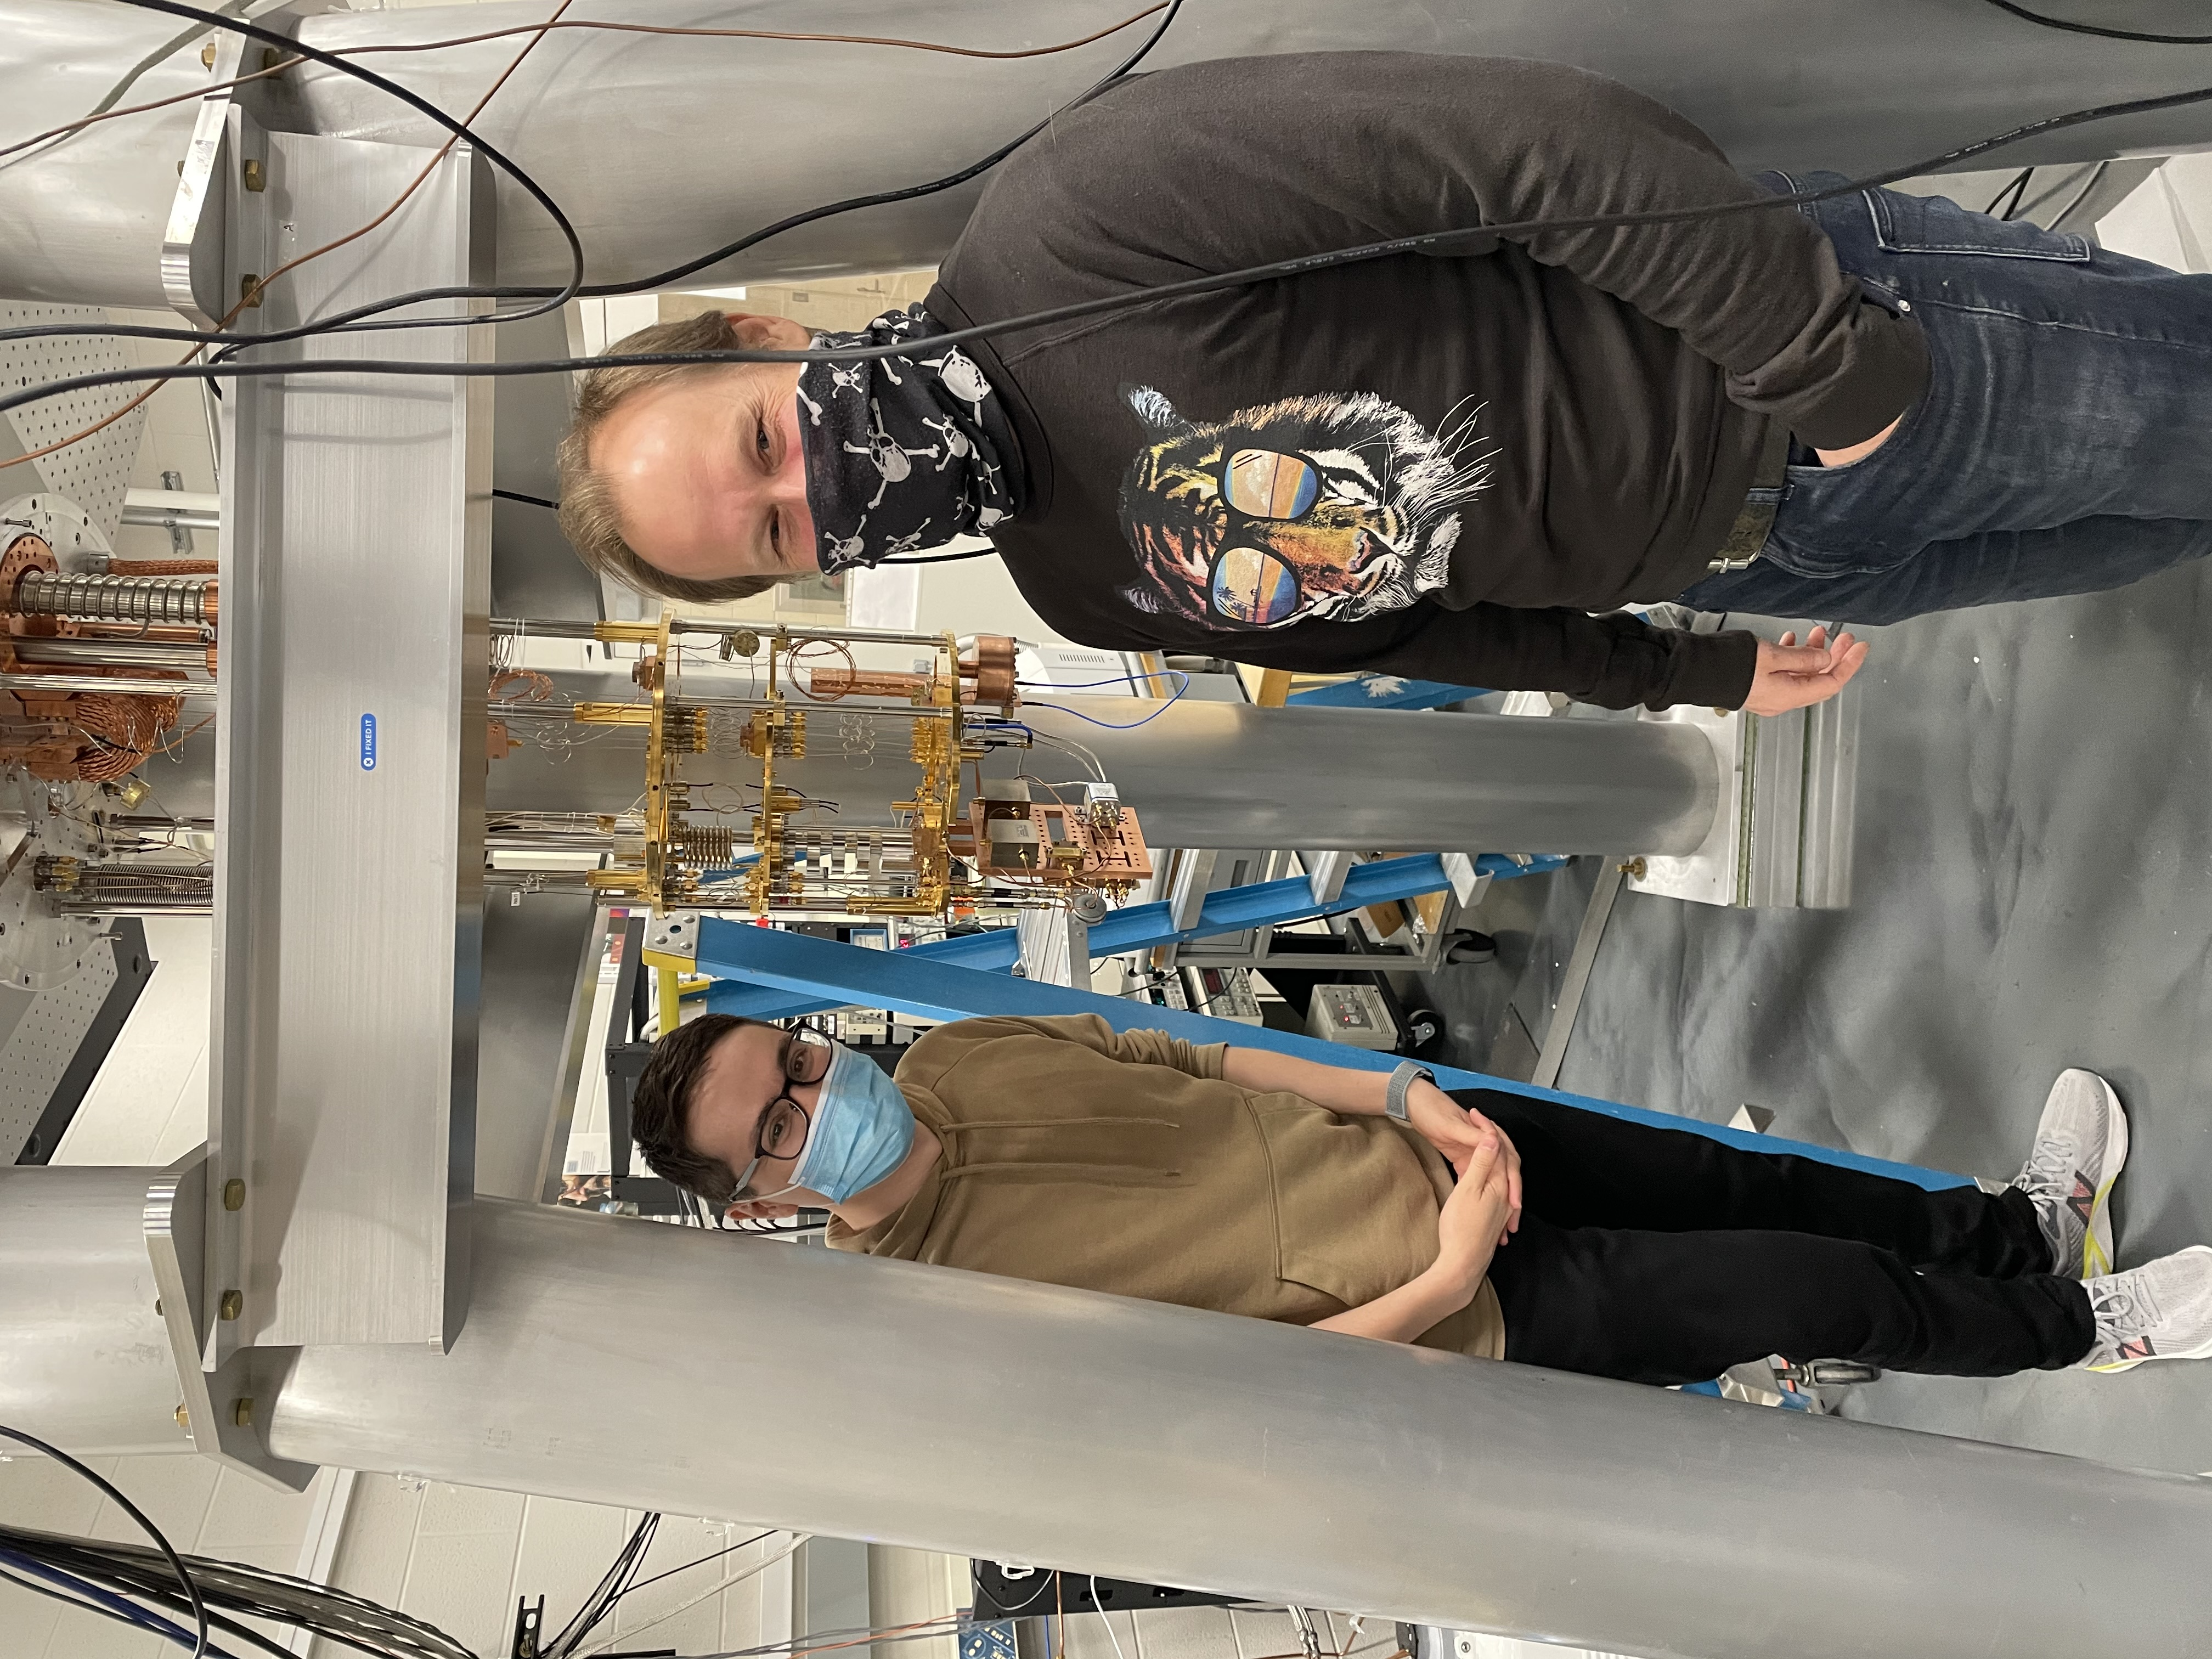
\includegraphics[width=1.3\textwidth]{qcfigures/lab.jpeg}}
      \end{center}
\end{columns}
      \end{footnotesize}
    }





\frame
    {
      \frametitle{Single electrons can make great qubits}
	
      \begin{footnotesize}
     \begin{columns}
       \column{5.0cm}

       At the heart is the trapping and control
       of individual electrons floating above pools of superfluid
       helium. These electrons form the qubits of our quantum
       computer, and the purity of the superfluid helium protects the
       intrinsic quantum properties of each electron. The  ultimate
       goal is to build a large-scale quantum computer based on
       quantum magnetic (spin) state of these trapped electrons.
\column{5cm}
      \begin{center}
	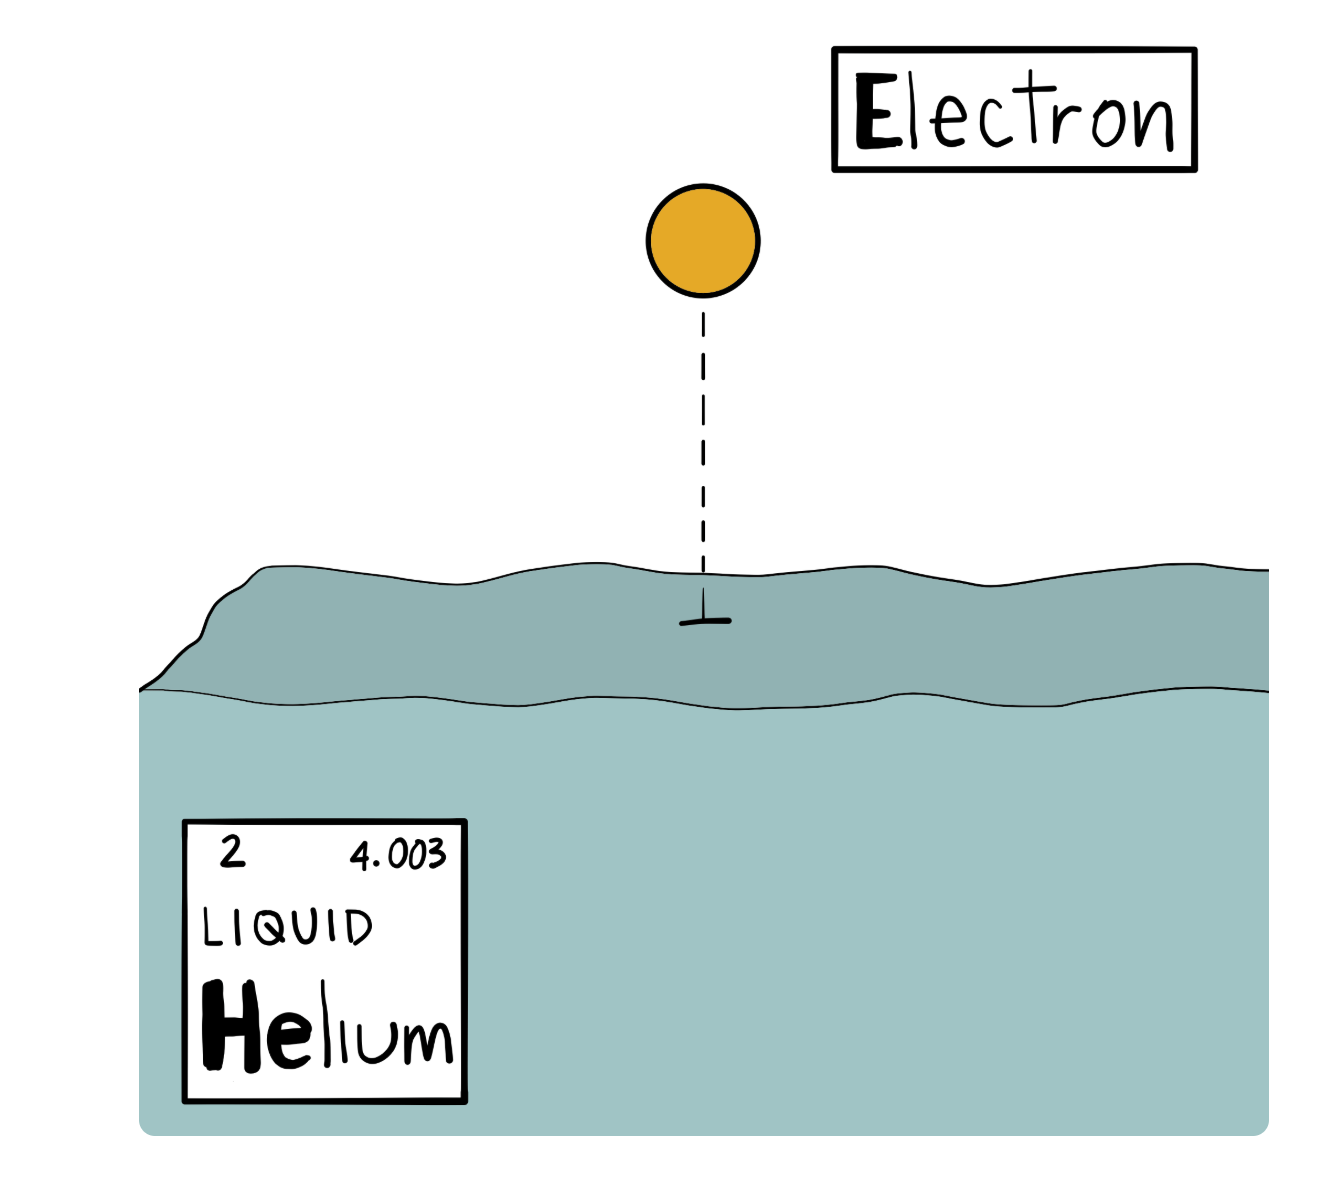
\includegraphics[width=1.2\textwidth]{qcfigures/nordicquantumfig1.png}
      \end{center}
\end{columns}
      \end{footnotesize}
    }


\frame
    {
      \frametitle{Trapping electrons in microchannels}
	
      \begin{footnotesize}
     \begin{columns}
       \column{5.0cm}
Microchannels fabricated into silicon wafers are filled with superfluid helium and energized electrodes. Together with the natural electron trapping properties of superfluid helium, these allow for the precision trapping of individual or multiple electrons. The microchannels are only a few micrometers in size, or about five times smaller than the diameter of a human hair.
\column{5cm}
      \begin{center}
	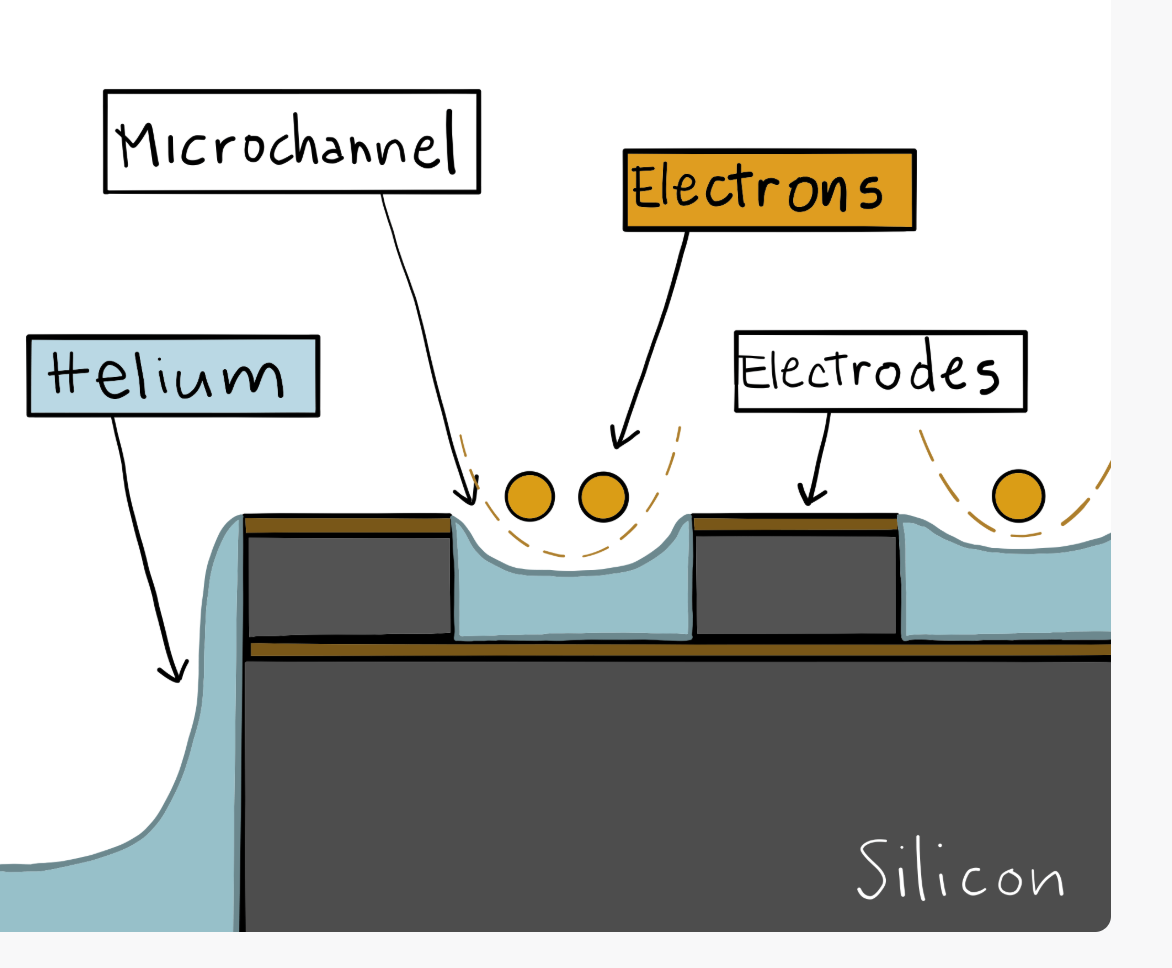
\includegraphics[width=1.2\textwidth]{qcfigures/nordicquantumfig2.png}
      \end{center}
\end{columns}
      \end{footnotesize}
    }

\frame
    {
      \frametitle{Control and readout}
	
      \begin{footnotesize}
     \begin{columns}
       \column{5.0cm}

       Microchannel regions can store thousands of electrons, from which one can be plucked and transported to the single electron control and readout area. In this region, microwave signals will interact with the electron to perform quantum logic gate operations, which will be readout via extremely fast electronics.


\column{5cm}
      \begin{center}
	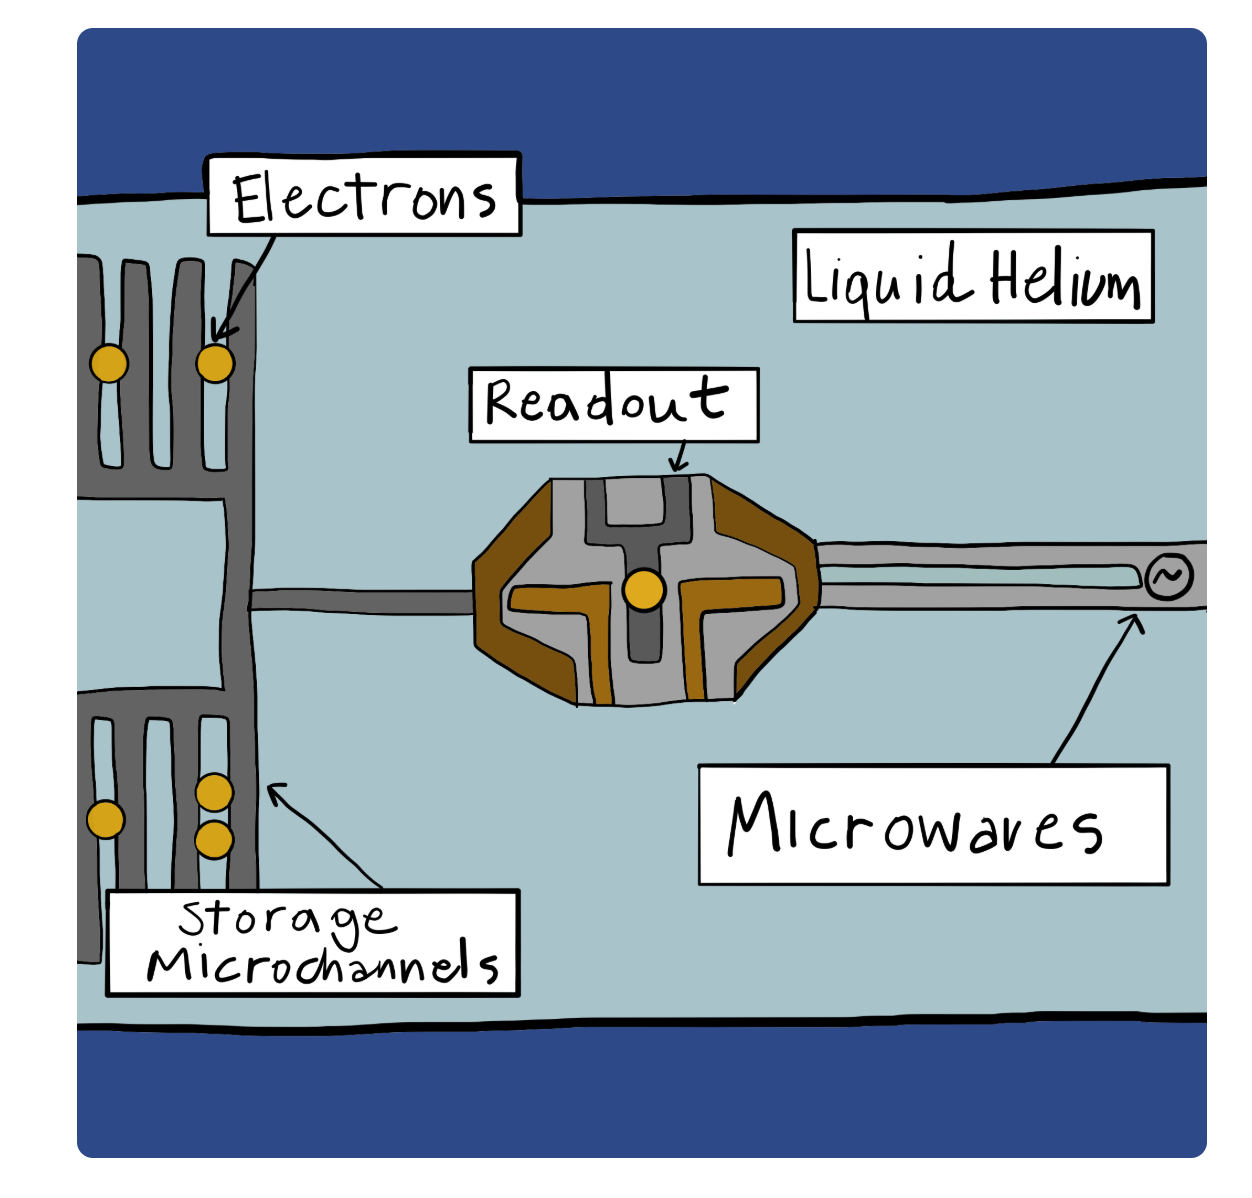
\includegraphics[width=1.2\textwidth]{qcfigures/nordicquantumfig3.png}
      \end{center}
\end{columns}
      \end{footnotesize}
    }


\frame
    {
      \frametitle{Operations for quantum computing}
	
      \begin{footnotesize}
     \begin{columns}
       \column{5.0cm}
Quantum information can be encoded in a number of ways using single electrons. Currently, we are working with the side-to-side(lateral) quantum motion of the electron in the engineered trap. This motion can either be in its lowest energy state, the ground state, or in a number of higher-energy excited states. This electron motion also provides the readout capabilities for the ultimate goal of building a large-scale quantum computer based on the electron's magnetic moment (spin).       
\column{5cm}
      \begin{center}
	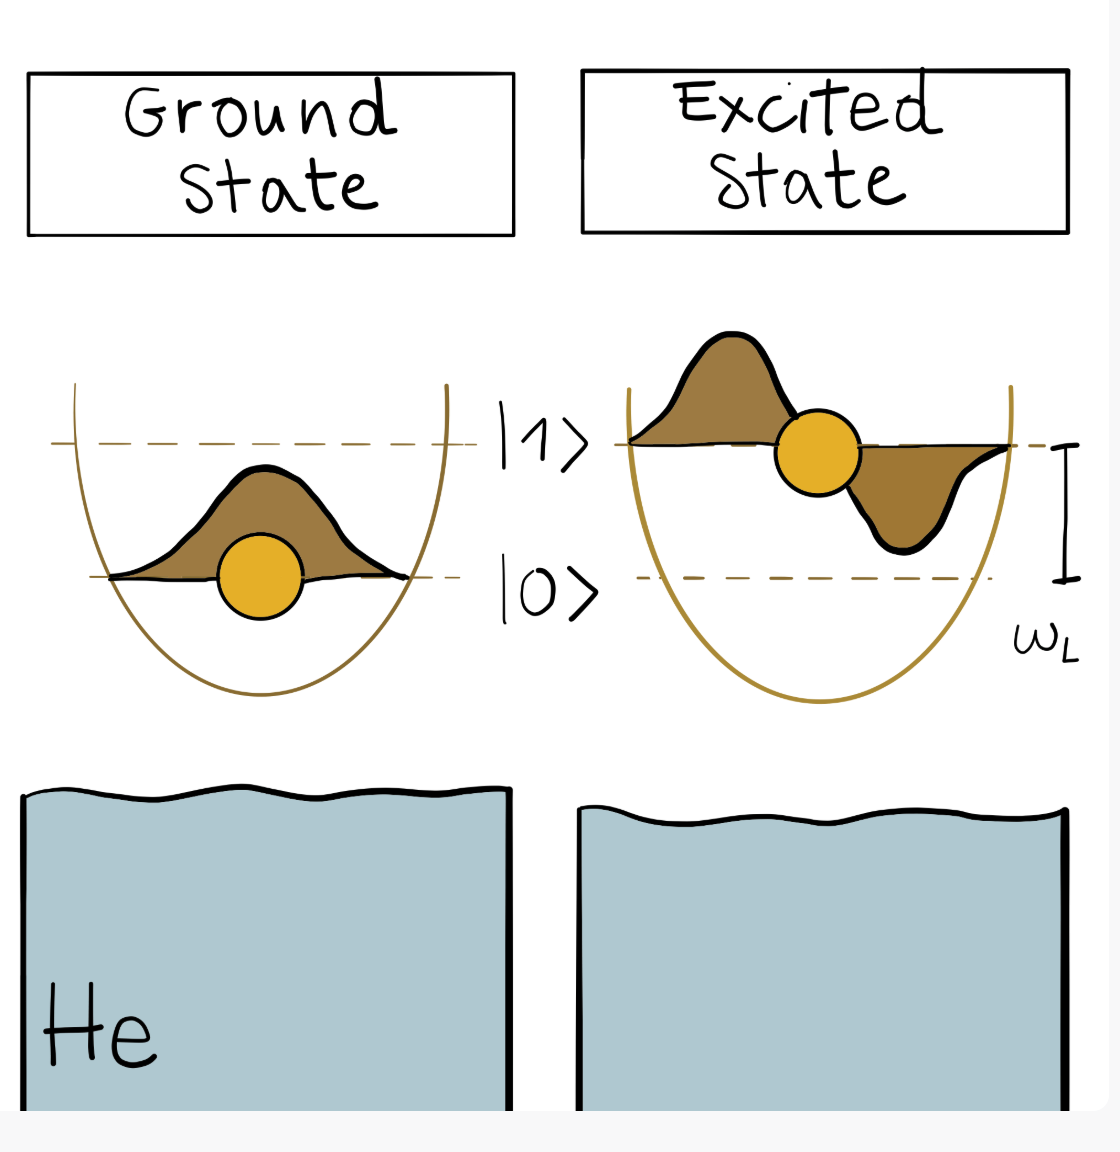
\includegraphics[width=1.2\textwidth]{qcfigures/nordicquantumfig4.png}
      \end{center}
\end{columns}
      \end{footnotesize}
    }
    
\section{Experiment and theory}




\begin{frame}[plain,fragile]
\frametitle{Qubit platforms}

\vspace{6mm}

% inline figure
\centerline{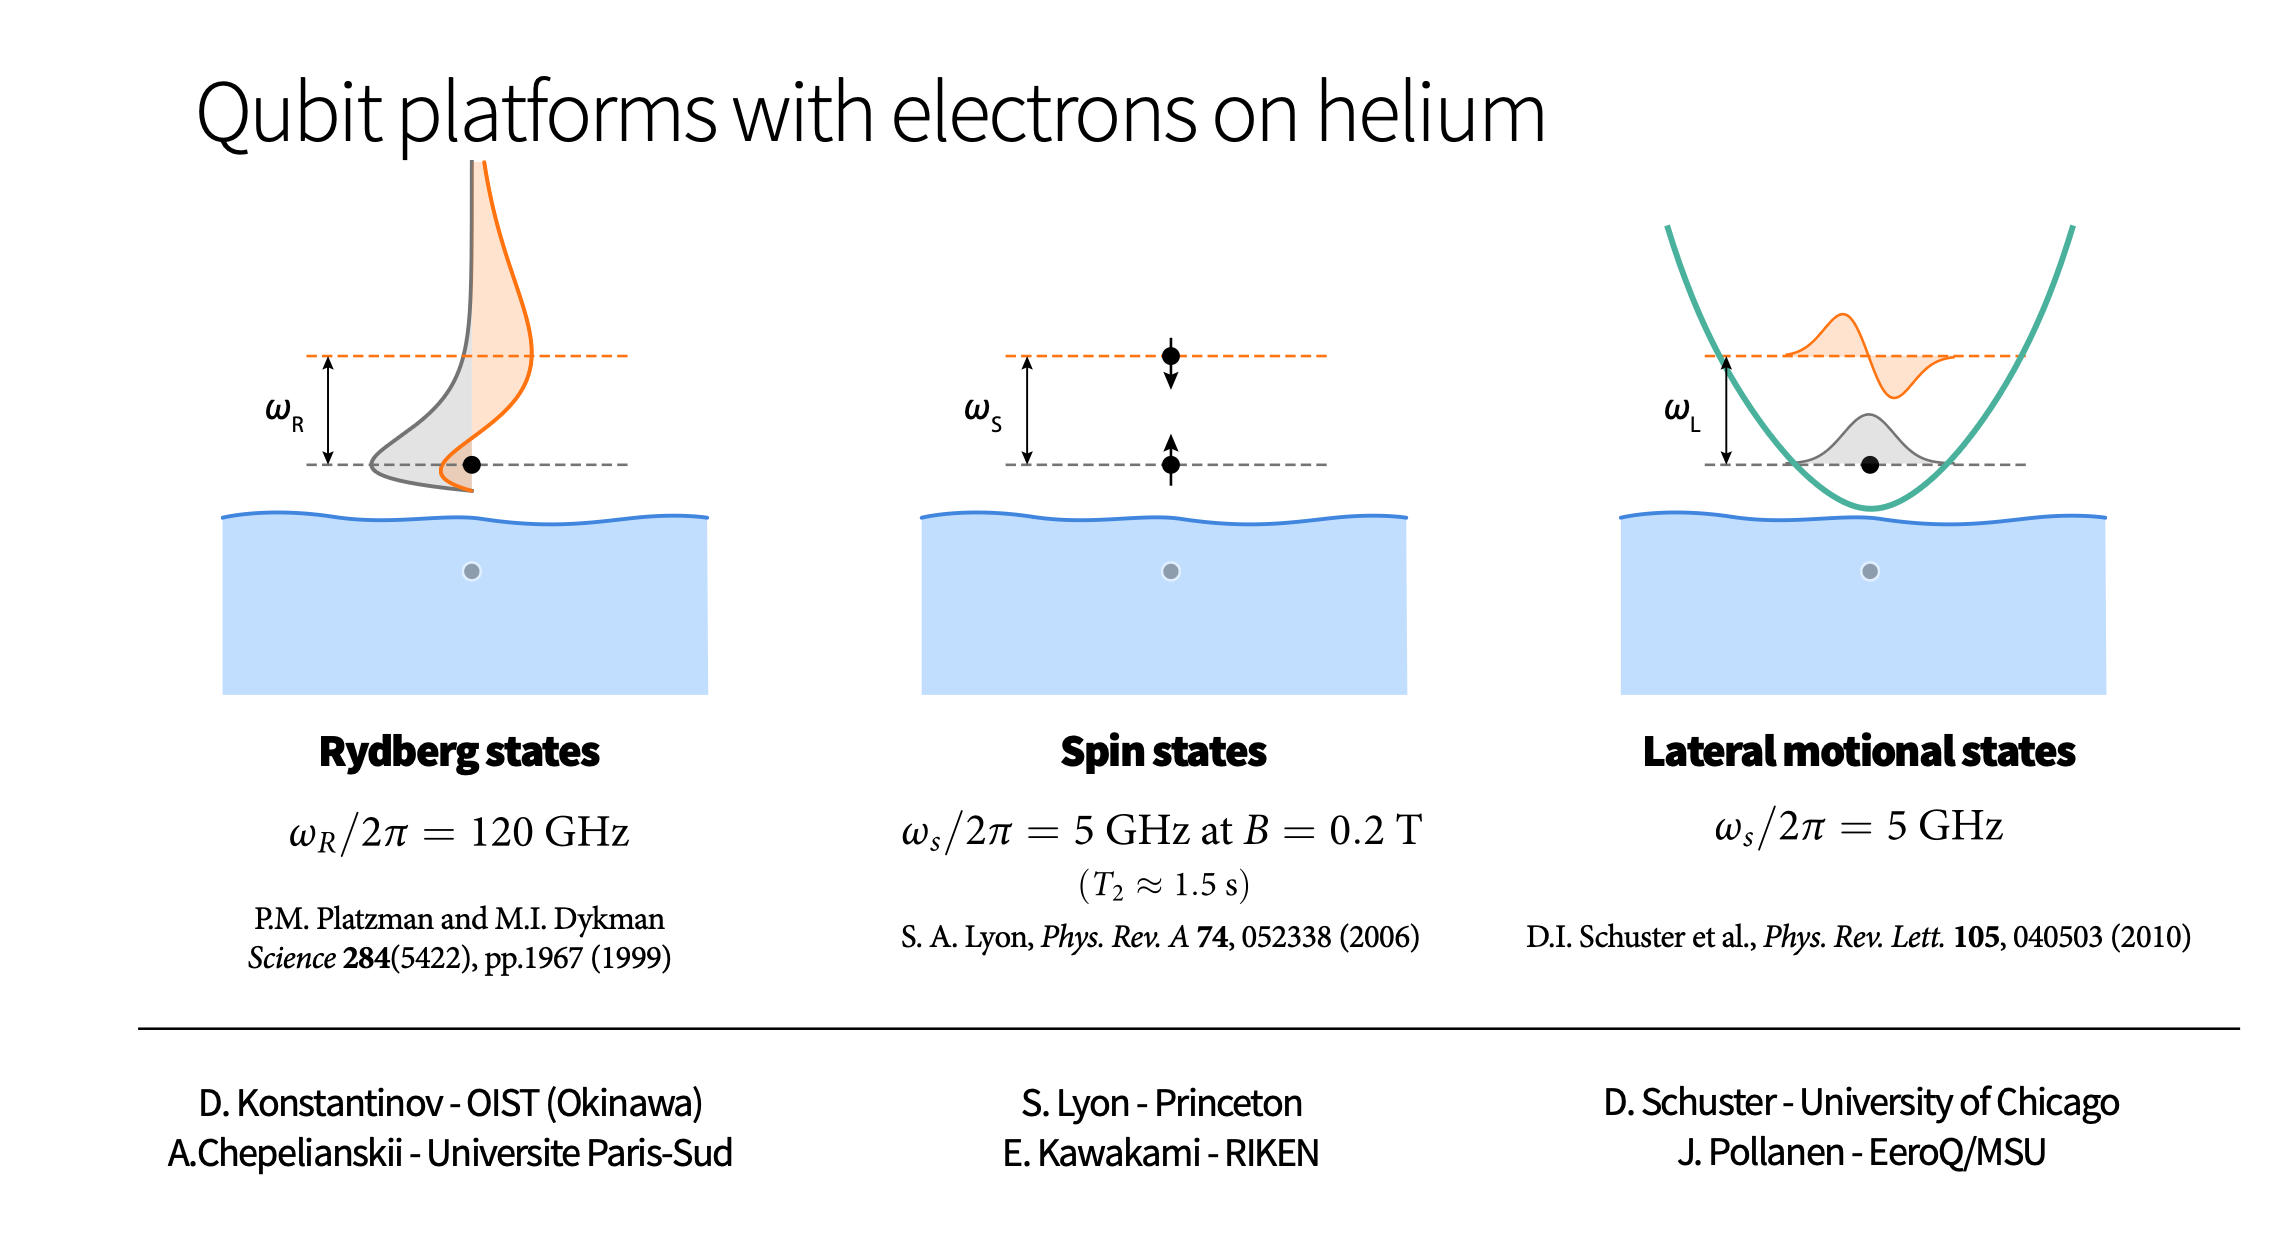
\includegraphics[width=1.2\linewidth]{qcfigures/Elhelium2.png}}

\vspace{6mm}
\end{frame}

\frame
    {
      \frametitle{Final experimental setup}
	
      \begin{footnotesize}
     \begin{columns}
       \column{5.0cm}
\begin{enumerate}
\item (a) Microdevice where two electrons are trapped in a double-well potential created by electrodes 1-7. The read-out is provided by two superconducting resonators dispersively coupled to  electron's in-plane motional states.

\item (b) Coupling constants from each individual electrode beneath the helium layer.

\item (c+d) The electron's energy in a  double-well electrostatic potential. 
\end{enumerate}

\column{6cm}
      \begin{center}
	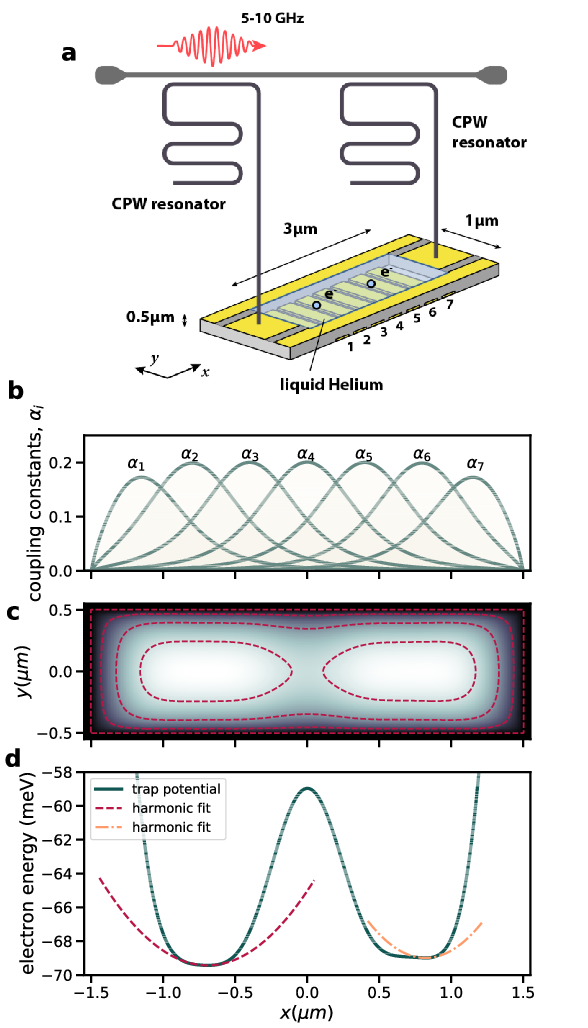
\includegraphics[width=0.65\textwidth]{qcfigures/figure1.png}
      \end{center}
\end{columns}
      \end{footnotesize}
    }







\begin{frame}[plain,fragile]
\frametitle{Export control}
\begin{table}
\begin{center}
\scalebox{.65}{
%{\footnotesize
\begin{tabular}{|l|l|l|} %{|l|p{3.5cm}|l|p{5.0cm}|}
\hline
\textbf{Technology/Component} & \textbf{Export Sensitivity Category} & \textbf{Reason for Sensitivity} \\
\hline
Superconducting CPW resonator (~6.04\,GHz) & Dual-Use (Quantum computing/EAR) & High-frequency superconducting circuit enabling dispersive qubit readout; advanced quantum sensor with potential defense/communications applications. \\
\hline
Single-electron trap (gated microchannel) &Dual-Use (Quantum hardware/EAR) & Precision single-electron trap for qubit storage and manipulation; specialized microelectronic architecture for quantum computing. \\
\hline
Superconducting electrodes (Nb films) &  Dual-Use (Superconducting electronics/EAR) & Superconducting materials in high-Q resonators and quantum circuits; key for low-loss quantum devices. \\
\hline
Pumped $^4$He cryostat (1.1\,K) &  Dual-Use (Cryogenic systems/EAR) & High-capacity cryogenic cooling enabling superconducting/qubit operation; cryogenic technology is often controlled (e.g. ECCN 3A904). \\
\hline
Superfluid $^4$He substrate &  Dual-Use (Cryogenic medium/EAR) & Specialized cryogenic environment for high-mobility electrons; a novel quantum material substrate with dual-use potential. \\
\hline
Cryogenic RF components  & Dual-Use (RF electronics/EAR) & GHz-range passive components in quantum measurement chain; similar hardware is used in radar and communications systems. \\
\hline
Low-noise RF amplifiers &  & Specialized amplifiers for weak-signal detection; critical in quantum readout and advanced electronic/sensor systems. \\
\hline
On-chip LC filters  & Dual-Use (RF filter technology/EAR) & Engineered filtering for high-frequency circuits; advanced RF integration relevant to communication and sensor devices. \\
\hline
Electron-on-helium qubit platform  & Dual-Use (Quantum computing/EAR) & Emerging quantum information platform targeted by new export controls; potential secure/advanced computation application. \\
\hline
\end{tabular}}
\end{center}
\end{table}


\end{frame}

% add slides about regulations of theory work


\end{document}



The US Bureau of Industry and Security (BIS) rules are new export
controls on certain quantum computing items, implemented through an
Interim Final Rule (IFR) on September 6, 2024. These rules add
worldwide licensing requirements for items on the Commerce Control
List (CCL), create a new license exception for allied countries, and
establish reporting requirements. The aim is to control the export of
advanced technologies, including quantum computing components,
software, and equipment, for national security and foreign policy
reasons.

Key aspects of the new rules



Key aspects of the new rules
Worldwide licensing: The controls apply to exports to all destinations, not just those restricted by the Country Chart.
License exception: A new exception, known as License Exception IEC, allows for exports to countries that have implemented equivalent controls, such as Italy, Canada, and the United Kingdom.
Control policy:There is a presumption of approval for exports to Country Group A:1 countries.There is a presumption of denial for exports to Country Groups D:1 and D:5 (such as China and Russia).Case-by-case reviews will be conducted for other countries.
Reporting requirements:
Companies must submit annual reports on certain exports and deemed exports, with a first report deadline of November 5, 2024, for the period of September 6 to October 28, 2024.
Termination reports are required within 30 days of an employee's or contractor's departure in certain situations.  

What is controlled?
Quantum computing items: This includes computers, software, components, materials, and related equipment used in their development and maintenance.
Advanced semiconductor manufacturing equipment: Tools and machines for producing advanced chips.
Gate All-Around Field-Effect Transistor (GAAFET) Technology: Technology for high-performance computing chips.
Additive manufacturing items: Equipment for producing metal components.



\begin{frame}[plain,fragile]
\frametitle{Observations (or conclusions if you prefer)}


\begin{block}{}
\begin{itemize}
\item How do we develop insights, competences, knowledge in AI and quantum technologies  that can advance a given field?
\begin{itemize}

  \item For example: Can we use ML to find out which correlations are relevant and thereby diminish the dimensionality problem in complex interacting  many-particle systems?

  \item Can we use AI/ML in detector analysis, accelerator design, analysis of experimental data and more?

  \item Can we use AL/ML to carry out reliable extrapolations by using current experimental knowledge and current theoretical models?
\item How do we study entanglement in various quantum platforms? Can we use AI/ML for better design?

\end{itemize}

\noindent
\item The community needs to invest in relevant educational efforts and training of scientists with knowledge in AI/ML and quantum technologies

\item Most likely tons of things I have forgotten
\end{itemize}

\noindent
\end{block}
\end{frame}

\begin{frame}{More conclusions or perspectives: Selected applications of Quantum Machine Learning}
\textbf{1. Quantum mechanical many-particle systems:}
\begin{itemize}
    \item Simulate  structures in nuclei, atoms, moleculs etc with QML.
\end{itemize}

\textbf{2. Finance:}
\begin{itemize}
    \item Quantum optimization for portfolio management.
\end{itemize}

\textbf{3. Image Recognition:}
\begin{itemize}
    \item Quantum-enhanced convolutional neural networks.
\end{itemize}
\end{frame}


\begin{frame}[plain,fragile]
\frametitle{Thank you for the attention and results from references in slides)}
\begin{enumerate}

\item Bryce Fore, Jane Kim, Morten Hjorth-Jensen, Alessandro Lovato, \textbf{Investigating the crust of neutron stars with neural-network quantum states}, Communications Physics \textbf{8}, 108  (2025) and \href{{https://www.nature.com/articles/s42005-025-02015-2}}{\nolinkurl{https://www.nature.com/articles/s42005-025-02015-2}}

\item Patrick Cook, Danny Jammooa, Morten Hjorth-Jensen, Daniel D. Lee, Dean Lee, \textbf{Parametric Matrix Models}, Nature Communications  under review and \href{{https://arxiv.org/abs/2401.11694}}{\nolinkurl{https://arxiv.org/abs/2401.11694}}

\item Niyaz R. Beysengulov, Johannes Pollanen, Øyvind S. Schøyen, Stian D. Bilek, Jonas B. Flaten, Oskar Leinonen, Håkon Emil Kristiansen, Zachary J. Stewart, Jared D. Weidman, Angela K. Wilson, Morten Hjorth-Jensen, Coulomb interaction-driven entanglement of electrons on helium, PRX Quantum 5, 030324 (2024) and \href{{https://journals.aps.org/prxquantum/abstract/10.1103/PRXQuantum.5.030324}}{\nolinkurl{https://journals.aps.org/prxquantum/abstract/10.1103/PRXQuantum.5.030324}}

\end{enumerate}
\end{frame}



\begin{frame}[plain,fragile]
\frametitle{Additional references)}
\begin{enumerate}

\item Jane Kim, Gabriel Pescia, Bryce Fore, Jannes Nys, Giuseppe Carleo, Stefano Gandolfi, Morten Hjorth-Jensen, Alessandro Lovato, \textbf{Neural-network quantum states for ultra-cold Fermi gases}, Communications Physics \textbf{7}, 148 (2024) and \href{{https://www.nature.com/articles/s42005-024-01613-w}}{\nolinkurl{https://www.nature.com/articles/s42005-024-01613-w}}

\item Bryce Fore, Jane M. Kim, Giuseppe Carleo, Morten Hjorth-Jensen, Alessandro Lovato, and Maria Piarulli, \textbf{Dilute neutron star matter from neural-network quantum states}, \href{{https://journals.aps.org/prresearch/abstract/10.1103/PhysRevResearch.5.033062}}{Physical Review  Research 5, 033062 (2023)}

\item Robert Solli, Daniel Bazin, Michelle P. Kuchera, Ryan R. Strauss, Morten Hjorth-Jensen, \emph{Unsupervised Learning for Identifying Events in Active Target Experiments}, \href{{https://www.sciencedirect.com/science/article/abs/pii/S0168900221004460}}{Nuclear Instruments and Methods in Physics Research Section A \textbf{1010}, 165461, (2020)}

\end{enumerate}
\end{frame}


\appendix{Additional material}






\begin{frame}{1. Quantum Support Vector Machines (QSVM)}
\textbf{Quantum Kernel Estimation:}
\begin{itemize}
    \item Maps classical data to a quantum Hilbert space.
    \item Quantum kernel measures similarity in high-dimensional space.
\end{itemize}

\pause
\textbf{Quantum Kernel:}
\[
K(x, x') = |\braket{\psi(x) | \psi(x')}|^2
\]

\textbf{Advantage:}
- Potentially exponential speedup over classical SVMs.
\end{frame}

\begin{frame}{2. Quantum Neural Networks (QNNs)}
\textbf{Quantum Neural Networks} replace classical neurons with parameterized quantum circuits.

\textbf{Key Concepts:}
\begin{itemize}
    \item Quantum Gates as Activation Functions.
    \item Variational Quantum Circuits (VQCs) for optimization.
\end{itemize}

\pause
\textbf{Parameterized Quantum Circuit:}
\[
U(\theta) = \prod_i R_y(\theta_i) \cdot CNOT \cdot R_x(\theta_i)
\]

\textbf{Advantage:}
- Quantum gradients enable exploration of non-convex landscapes.
\end{frame}

\begin{frame}{3. Quantum Boltzmann Machines (QBMs)}
\textbf{Quantum Boltzmann Machines} leverage quantum mechanics to sample from a probability distribution.

\begin{itemize}
    \item Quantum tunneling aids in escaping local minima.
    \item Quantum annealing for optimization problems.
\end{itemize}

\pause
\textbf{Quantum Hamiltonian:}
\[
H = -\sum_i b_i \sigma_i^z - \sum_{ij} w_{ij} \sigma_i^z \sigma_j^z
\]

\textbf{Advantage:}
- Efficient sampling in complex probability distributions.
\end{frame}


\section{Future Perspectives}
\begin{frame}{Future Perspectives in QML}
\textbf{1. Fault-Tolerant Quantum Computing:}
\begin{itemize}
    \item Overcoming noise for stable quantum circuits.
\end{itemize}

\textbf{2. Hybrid Quantum-Classical Models:}
\begin{itemize}
    \item Combining quantum circuits with classical neural networks.
\end{itemize}

\textbf{3. Quantum Internet:}
\begin{itemize}
    \item Distributed quantum machine learning over quantum networks.
\end{itemize}
\end{frame}
















\begin{frame}[plain,fragile]
\frametitle{Universal approximation theorem}

The universal approximation theorem plays a central role in deep
learning.  \href{{https://link.springer.com/article/10.1007/BF02551274}}{Cybenko (1989)} showed
the following:

\begin{block}{}
Let $\sigma$ be any continuous sigmoidal function such that
\[
\sigma(z) = \left\{\begin{array}{cc} 1 & z\rightarrow \infty\\ 0 & z \rightarrow -\infty \end{array}\right.
\]
Given a continuous and deterministic function $F(\bm{x})$ on the unit
cube in $d$-dimensions $F\in [0,1]^d$, $x\in [0,1]^d$ and a parameter
$\epsilon >0$, there is a one-layer (hidden) neural network
$f(\bm{x};\bm{\Theta})$ with $\bm{\Theta}=(\bm{W},\bm{b})$ and $\bm{W}\in
\mathbb{R}^{m\times n}$ and $\bm{b}\in \mathbb{R}^{n}$, for which
\[
\vert F(\bm{x})-f(\bm{x};\bm{\Theta})\vert < \epsilon \hspace{0.1cm} \forall \bm{x}\in[0,1]^d.
\]

\end{block}
\end{frame}

\begin{frame}[plain,fragile]
\frametitle{The approximation theorem in words}

\textbf{Any continuous function $y=F(\bm{x})$ supported on the unit cube in
$d$-dimensions can be approximated by a one-layer sigmoidal network to
arbitrary accuracy.}

\href{{https://www.sciencedirect.com/science/article/abs/pii/089360809190009T}}{Hornik (1991)} extended the theorem by letting any non-constant, bounded activation function to be included using that the expectation value
\[
\mathbb{E}[\vert F(\bm{x})\vert^2] =\int_{\bm{x}\in D} \vert F(\bm{x})\vert^2p(\bm{x})d\bm{x} < \infty.
\]
Then we have
\[
\mathbb{E}[\vert F(\bm{x})-f(\bm{x};\bm{\Theta})\vert^2] =\int_{\bm{x}\in D} \vert F(\bm{x})-f(\bm{x};\bm{\Theta})\vert^2p(\bm{x})d\bm{x} < \epsilon.
\]
\end{frame}

\begin{frame}[plain,fragile]
\frametitle{More on the general approximation theorem}

None of the proofs give any insight into the relation between the
number of of hidden layers and nodes and the approximation error
$\epsilon$, nor the magnitudes of $\bm{W}$ and $\bm{b}$.

Neural networks (NNs) have what we may call a kind of universality no matter what function we want to compute.

\begin{block}{}
It does not mean that an NN can be used to exactly compute any function. Rather, we get an approximation that is as good as we want. 
\end{block}
\end{frame}

\begin{frame}[plain,fragile]
\frametitle{Class of functions we can approximate}

\begin{block}{}
The class of functions that can be approximated are the continuous ones.
If the function $F(\bm{x})$ is discontinuous, it won't in general be possible to approximate it. However, an NN may still give an approximation even if we fail in some points.
\end{block}
\end{frame}

\end{document}

%-----------------------------------------------------------
\section{Future Perspectives}
\begin{frame}{Future Perspectives}
\textbf{Quantum Internet:}
\begin{itemize}
    \item Entanglement as a resource for global quantum networks.
\end{itemize}

\textbf{Fault-Tolerant Quantum Computing:}
\begin{itemize}
    \item Quantum error correction leveraging entanglement.
\end{itemize}

\textbf{Advanced Quantum Sensors:}
\begin{itemize}
    \item Improved sensitivity for medical and scientific applications.
\end{itemize}

\pause
\textbf{Conclusion:}
- Quantum entanglement is a fundamental resource.  
- It enables quantum supremacy in communication, computation, and sensing.
\end{frame}







Based on a detailed review of the article **“Strong coupling of a microwave photon to an electron on helium” (arXiv:2509.14506v1)** and its supplementary materials, the **technological components potentially subject to export control regulations** (such as under the U.S. **Export Administration Regulations (EAR)**, EU **Dual-Use Regulation (EU) 2021/821**, or Norwegian equivalents) are the following:

---

### **1. Superconducting Quantum Microwave Devices**

* **High-impedance superconducting resonator** (fabricated from **titanium nitride (TiN)** and **niobium (Nb)** nanowires).

  * These are **superconducting microwave resonators** designed for strong coupling to quantum systems.
  * Controlled under export lists when used in **quantum computing**, **high-frequency detection**, or **quantum-limited measurement** systems (ECCN 3A991/3A231 or EU Category 3A001.b.10).

---

### **2. Quantum Control and Measurement Electronics**

* **Cryogenic microwave circuitry** including high-electron mobility transistor (**HEMT**) amplifiers, **bias tees**, and **microwave filters** capable of operation below 10 mK.

  * Such systems are part of **quantum-limited cryogenic readout** chains for qubit measurement and can fall under export controls as **quantum-limited amplifiers** or **quantum sensing components**.

---

### **3. Quantum Dot and Trapping System**

* **Electrostatic trapping and control of single electrons on superfluid helium**, integrated into a **microfabricated silicon-based microfluidic platform**.

  * These devices implement **quantum confinement** and **precision charge control**, key enabling technologies for **quantum information processing**.
  * Falls under **dual-use classification for quantum information systems** (ECCN 3E001 or EU 3E001, technology for the development of quantum computing devices).

---

### **4. Fabrication and Design Technology**

* **Electron-beam lithography and reactive-ion etching (RIE) methods** for patterning TiN/Nb superconducting circuits with sub-micrometer resolution.

  * Such fabrication know-how and associated CAD/FEM simulation tools (e.g., finite element models of qubit–resonator coupling) may be classified under **3E002** (“technology for development or production of superconducting electronics”).

---

### **5. Cryogenic and Quantum Experimental Systems**

* **Dilution refrigerator systems (Bluefors LD400)** operating below 10 mK with integrated **quantum microwave lines**, filters, and bias systems.

  * While the refrigerator itself is not normally export-restricted, **integration into quantum computing or quantum sensing architectures** may invoke **dual-use provisions**.

---

### **Summary of Export-Relevant Elements**

| Category                         | Component                                                            | Potential Control Reference |
| -------------------------------- | -------------------------------------------------------------------- | --------------------------- |
| Superconducting quantum circuits | TiN/Nb high-impedance resonators                                     | 3A991.b.2 / 3A231           |
| Quantum control electronics      | Cryogenic HEMT amplifiers, bias tees, low-noise microwave components | 3A001.b.10                  |
| Quantum devices                  | Electron-on-helium quantum dots and coupling schemes                 | 3E001 / 3E002               |
| Fabrication technology           | E-beam lithography, RIE, FEM-based quantum design                    | 3E002                       |
| Cryogenic systems                | Dilution refrigerator integration with quantum hardware              | 3B001 or “use” under 3E001  |

---

### **Non-Controlled Scientific Aspects**

The *scientific data, published results,* and *basic research* aspects of this work—such as theoretical models, FEM simulations, and open-source software repositories (e.g., **ZeroHeliumKit**, **Quantum Electron**)—are **not subject to export control** under the research exemption for publicly available fundamental research.

---

Would you like me to prepare a **one-page summary table** (formatted for a grant or compliance document) that clearly lists these components, control categories, and justifications?



Here’s a **one-page summary table** outlining the **technological components in the article** *“Strong coupling of a microwave photon to an electron on helium” (arXiv:2509.14506v1)* that may be influenced by **export control regulations** (e.g., EU Dual-Use Regulation 2021/821, EAR, or Norwegian equivalents).

---

## **Export Control Summary – Technological Components in “Strong Coupling of a Microwave Photon to an Electron on Helium”**

| **Category**                             | **Component / Technology**                                                          | **Description and Use**                                                                                                     | **Potential Export Control Relevance**                                                                                          | **Indicative Control Reference**        |
| ---------------------------------------- | ----------------------------------------------------------------------------------- | --------------------------------------------------------------------------------------------------------------------------- | ------------------------------------------------------------------------------------------------------------------------------- | --------------------------------------- |
| **1. Superconducting Quantum Circuits**  | High-impedance **TiN/Nb superconducting resonators**                                | Nanofabricated microwave resonators enabling strong coupling between single electrons and photons at GHz frequencies.       | Considered **quantum-limited superconducting electronics**; restricted when used for quantum computing or sensing applications. | EU 3A001.b.10 / EAR 3A991.b.2 or 3A231  |
| **2. Quantum Control Electronics**       | **Cryogenic microwave electronics** (HEMT amplifiers, bias tees, filters, mixers)   | Low-noise signal generation and readout below 10 mK; critical for qubit control and quantum-limited detection.              | Controlled as **quantum-measurement and control components** with ultra-low-temperature performance.                            | EU 3A001.b.10 / EAR 3A991.b.2           |
| **3. Quantum Device Platform**           | **Electron-on-helium microtrap**                                                    | Electrostatic confinement of single electrons on superfluid helium; prototype for charge-qubit or spin-qubit architectures. | Falls under **quantum-information hardware development**; controlled if intended for computing or encryption applications.      | EU 3E001 / EAR 3E001                    |
| **4. Fabrication and Design Technology** | **E-beam lithography, RIE, CAD/FEM simulation tools** for superconducting circuits  | Sub-micron fabrication and simulation of qubit–resonator coupling and device geometry.                                      | Considered **technology for production/development of superconducting quantum devices**.                                        | EU 3E002 / EAR 3E002                    |
| **5. Cryogenic Infrastructure**          | **Dilution refrigerator systems (≤ 10 mK)** integrated with quantum microwave lines | Enables operation of superconducting and electron-on-helium systems in the quantum regime.                                  | Not controlled as standalone equipment, but regulated when integrated into **quantum computing or sensing systems**.            | EU 3B001 / EAR 3E001 (“use” technology) |
| **6. Non-Controlled Research Elements**  | Published **theoretical models, open-source code, and data**                        | Publicly available fundamental research outputs (e.g., simulations, publications).                                          | **Exempt from export controls** under the public-domain / fundamental-research exemption.                                       | EU Art. 1(2) / EAR §734.8               |

---

**Summary:**
The export-relevant elements in this work mainly concern *superconducting microwave devices, cryogenic quantum control electronics,* and *microfabricated quantum systems* that enable manipulation of single electrons. Associated design and fabrication know-how may also fall under dual-use categories. Purely theoretical and published research outputs remain outside export control.

---

Would you like me to generate this as a **formatted one-page PDF table** (e.g., for inclusion in a compliance or grant appendix)?



Based on the detailed review of the uploaded paper **“Universal Control of a Semiconductor Spin Qubit using Electron Spin Resonance” (arXiv:2509.13946v2)**, the following **technological components** described or implied in the work are **potentially influenced by export control regulations** (notably under the **EU Dual-Use Regulation 2021/821**, **U.S. EAR**, and corresponding **Norwegian export control framework**).

---

## **Technological Components Potentially Subject to Export Controls**

| **Category**                                   | **Component / Technology**                                                                   | **Description and Function**                                                                                           | **Export Control Relevance**                                                                                                                   | **Indicative Control Reference**             |
| ---------------------------------------------- | -------------------------------------------------------------------------------------------- | ---------------------------------------------------------------------------------------------------------------------- | ---------------------------------------------------------------------------------------------------------------------------------------------- | -------------------------------------------- |
| **1. Quantum Device Platform**                 | **Semiconductor spin qubit in Si/SiGe heterostructure**                                      | Quantum dot device confining single electrons in isotopically purified silicon, used for spin-based qubit realization. | Considered **quantum information processing hardware**; controlled when used or developed for quantum computation or secure communication.     | EU 3E001 / EAR 3E001                         |
| **2. Microwave Spin Control Hardware**         | **On-chip microwave transmission lines / ESR control antennas**                              | Nanofabricated gate electrodes deliver microwave magnetic fields for electron spin resonance (ESR) control.            | May fall under controls for **high-frequency quantum control electronics** and **superconducting/semiconducting microwave circuits**.          | EU 3A001.b.10 / EAR 3A991.b.2                |
| **3. Cryogenic Quantum Control System**        | **Cryogenic measurement setup with dilution refrigerator (<10 mK)**                          | Enables qubit initialization, coherent control, and readout under quantum-coherent conditions.                         | Standalone refrigeration systems are not controlled, but **integrated cryogenic quantum systems** may be dual-use.                             | EU 3B001 / EAR 3E001 (“use” technology)      |
| **4. Qubit Readout Electronics**               | **RF reflectometry and charge sensing circuits (SET-based)**                                 | High-sensitivity charge detectors and RF amplifiers used to measure single-spin states.                                | Controlled under **quantum-limited measurement and sensing electronics**.                                                                      | EU 3A001.b.10 / EAR 3A991                    |
| **5. Fabrication and Design Technology**       | **E-beam lithography, atomic layer deposition (ALD), and etching for Si/SiGe qubit devices** | Processes to pattern gate-defined quantum dots and heterostructures with nanometer precision.                          | Falls under **technology for the development or production of quantum or semiconductor devices**.                                              | EU 3E002 / EAR 3E002                         |
| **6. Quantum Control Software and Algorithms** | **Pulse sequences, calibration routines, and control optimization software**                 | Numerical optimization of ESR pulses and gate voltages for coherent spin rotations.                                    | If made publicly available as fundamental research, *not controlled*; otherwise, classified as **technology for quantum information systems**. | EU 3E001 (if proprietary) / Exempt if public |
| **7. Quantum Measurement Infrastructure**      | **Low-noise cryogenic amplifiers (HEMT), RF filters, and bias circuitry**                    | Quantum-limited amplifiers and filters enabling high-fidelity qubit readout.                                           | Controlled for **quantum-limited cryogenic readout systems** used in quantum computing or metrology.                                           | EU 3A001.b.10 / EAR 3A991.b.2                |
| **8. Cleanroom Facilities & Know-how**         | **Semiconductor device integration and heterostructure growth methods (MBE, CVD)**           | Growth and processing of isotopically enriched Si/SiGe layers and metallic gates for qubit fabrication.                | Controlled under **semiconductor manufacturing technology** when tied to quantum or spin-based computing development.                          | EU 3E002 / EAR 3E002                         |

---

### **Non-Controlled Scientific Aspects**

* **Published results**, **theoretical models**, and **open data or software** released through public repositories are **not subject to export control**, consistent with the *fundamental research exemption* (EU Regulation 2021/821, Art. 1(2); EAR §734.8).
* Dissemination of *educational or basic research results* does not require export authorization unless tied to proprietary or classified technologies.

---

### **Summary**

The components most relevant to export controls are:

* **Quantum dot devices and spin qubit architectures (3E001)**
* **Microwave ESR control electronics (3A001.b.10)**
* **Cryogenic readout systems (3A991.b.2)**
* **Fabrication and process know-how (3E002)**

These are all **dual-use technologies**, potentially regulated if exported outside the EU/Norway for quantum computing or secure communication purposes.

---

Would you like me to format this information as a **one-page PDF summary table**, similar to the earlier QONTROL export control document?
